% ==================================================================================================================================
% Théorie des Langages

% - - - - - - - - - - - - - - - - - - - - - - - - - 
%                       TITLE
% - - - - - - - - - - - - - - - - - - - - - - - - - 


% - - - - - - - - - - - - - - - - - - - - - - - - - 
%               Chapters Inclusion
% - - - - - - - - - - - - - - - - - - - - - - - - - 

\chapter{Théorie des Graphes}

\minitoc 

% ==================================================================================================================================
% Introduction

\emph{Fiche réalisée grâce au cours de Thierry Montaut et Laura Brillon.}

Dans ce cours, on note $G = (X,E)$ un graphe.

% ==================================================================================================================================
% Graphes, Représentations et Parcours

\section{Graphes, Représentations et Parcours}

\subsection{Définitions - Graphes Orientés et Non Orientés}

\subsubsection{Vocabulaire}

\begin{definition}[Graphe non orienté]
    On appelle graphe non orienté un couple d'ensembles finis $G = (X,E)$ où $X = \{1, \dots, n\}$ représente les sommets du graphe
    et $E = \{ (x_i, y_j), \dots \}, x_i, y_j \in X$ l'ensemble des arrêtes du graphe. Une arrête est une liaison entre deux sommets.

    Un graphe est dit \textbf{simple} s'il n'existe pas de double arrêtes entre deux sommets ou de bouble (i.e une arrête de la forme $(x,x)$).
    Autrement, on parle de \textbf{multigraphe.}
\end{definition}

\begin{definition}[Graphe Orienté]
    On appelle graphe orienté un couple d'ensembles finis $G = (X,E)$ où $X = \{1, \dots, n\}$ représente les sommets du graphe 
    et $E = \{ (x_i, y_j), \dots \}$, $ x_i, y_j \in X$ l'ensemble ordonné des arrêtes du graphe. 
    Pour un graphe orienté, les notions de graphe simple et multiraphe sont les même que pour le cas non orienté.
\end{definition}

\begin{example}[Graphes et leur représentation graphique]
    Soient $G_1$ et $G_2$ deux graphes, en voici une représentation :
    \begin{figure}[h]
        \centering
        \begin{minipage}{0.45\textwidth}  % Première image dans 45% de la largeur de la page
          \centering
          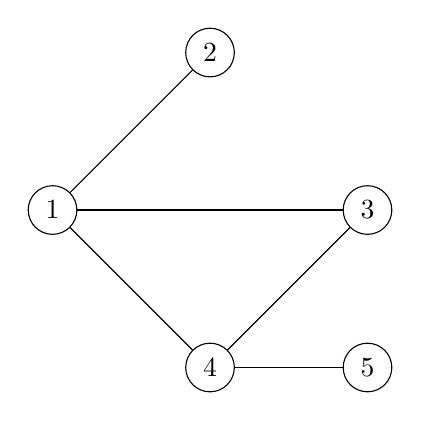
\begin{tikzpicture}[scale=1]
            % Déclaration des sommets avec des cercles
            \node[draw, circle] (1) at (0,0) {1};
            \node[draw, circle] (2) at (2,2) {2};
            \node[draw, circle] (3) at (4,0) {3};
            \node[draw, circle] (4) at (2,-2) {4};
            \node[draw, circle] (5) at (4,-2) {5};
      
            % Ajout des arêtes (non orientées)
            \draw (1) -- (2);
            \draw (1) -- (3);
            \draw (1) -- (4);
            \draw (4) -- (5);
            \draw (3) -- (4);
          \end{tikzpicture}
          \caption{Graphe non orienté}
          \label{fig:non-oriente}
        \end{minipage}%
        \hfill % Ajoute de l'espace flexible entre les deux images
        \begin{minipage}{0.45\textwidth}  % Deuxième image dans 45% de la largeur de la page
          \centering
          \begin{tikzpicture}[->,>=stealth',shorten >=1pt,auto,node distance=2cm,thick,scale=1]
            % Déclaration des sommets avec des cercles
            \node[draw, circle] (1) at (0,0) {1};
            \node[draw, circle] (2) at (2,2) {2};
            \node[draw, circle] (3) at (4,0) {3};
            \node[draw, circle] (4) at (2,-2) {4};
            \node[draw, circle] (5) at (4,-2) {5};
      
            % Ajout des arêtes orientées
            \draw[->] (1) -- (2);
            \draw[->] (1) -- (3);
            \draw[->] (4) -- (1);
            \draw[->] (2) -- (4);
            \draw[->] (3) -- (5);
          \end{tikzpicture}
          \caption{Graphe orienté}
          \label{fig:oriente}
        \end{minipage}
      \end{figure}
\end{example}

\begin{definition}[Planaire]
    Une graphe $G$ est dit planaire s'il existe une représentation de $G$ 
    en deux dimensions telle qu'aucun de ses sommets ne se croisent.
\end{definition}


\subsubsection{Voisinnage et degré}

\begin{definition}[Voisinnage]
    Le voisinnage d'un sommet $x$ de $G$ est l'ensemble des sommets $y$ de $G$ tels qu'il existe une arrête entre $x$ et $y$ dans $G$.
    On le note $V(x)$.
\end{definition}

\begin{remark}
    Si $x$ est dans le voisinnage de $y$, on dira que $x$ est adlascent à $y$ et inversement.
\end{remark}

\begin{definition}[Degré]
    Le degré d'un sommet $x$ de $G$ est le cardinal du voisinnage $x$. On le note $d(x)$.
    Un sommet de voisinnage nul est dit \textbf{isolé} et un sommet de voisinnage égal à 1 est dit \textbf{pendant}.
\end{definition}

\begin{definition}[Voisinnage entrant et sortant]
    Soit $G$ un graphe orienté et $x$ un sommet de $G$. On définit deux types de voisinnages :
    \begin{itemize}
        \item \textbf{Voisinnage entrant :} noté $V^-(X)$ est l'ensemble des prédécesseurs de $x$.
        \item \textbf{Voisinnage sortant :} noté $V^+(X)$ est l'ensemble des successeurs de $x$.
    \end{itemize}
    On définira comme précédemment le degré sortant et le degré entrant d'un sommet $x$.
\end{definition}


\subsubsection{Graphes Remarquables (non orientés)}

Dans cette sous-section, nous ne parlerons que de graphes non-orientés.

\begin{definition}[Graphe complet]
    On appelle graphe complet un graphe tel que pour tous sommets $x$ et $y$ de $G$ il existe une arrête entre $x$ et $y$ dans $G$.
    Les graphes complets $n$ sommets sont notés $K_n$
\end{definition}

\begin{remark}
    Autre définition de graphe complet et un petit peu d'histoire ne fera pas mal...
    \begin{itemize}
        \item On peut aussi définir un graphe complet comme étant un graphe dont tous ses sommets sont adjascents.
        \item  \emph{La notation $K$ pourrait avoir deux origines, la première étant en hommage à Kazimierz Kuratowski, 
        un éminent mathématiciens polonais ayant beaucoup contribué à la théorie des graphes. La seconde, plus simple, $K$
        proviendrait de sa traduction en Allemand komplett.}
    \end{itemize}
\end{remark}

\begin{example}
    Représentation des graphes complets $K_4$ et $K_5$ :
    \begin{figure}[h]
        \centering
        \begin{minipage}{0.45\textwidth}  % Première image dans 45% de la largeur de la page
            \centering
            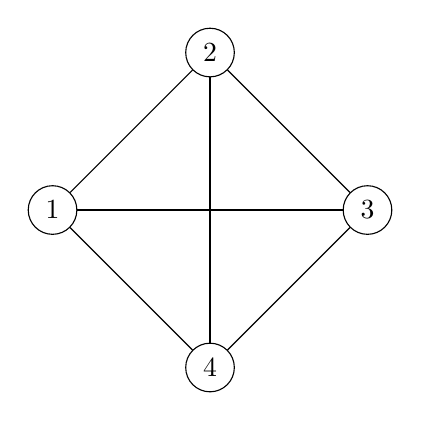
\begin{tikzpicture}[scale=1]
                % Déclaration des sommets avec des entiers pour K4
                \node[draw, circle] (1) at (0, 0) {1};
                \node[draw, circle] (2) at (2, 2) {2};
                \node[draw, circle] (3) at (4, 0) {3};
                \node[draw, circle] (4) at (2, -2) {4};
            
                % Ajout des arêtes pour K4 (chaque sommet est connecté aux autres)
                \draw (1) -- (2);
                \draw (1) -- (3);
                \draw (1) -- (4);
                \draw (2) -- (3);
                \draw (2) -- (4);
                \draw (3) -- (4);
              \end{tikzpicture}
              \caption{Graphe complet \( K_4 \)}
              \label{fig:K4-entiers}
        \end{minipage}
        \hfill % Ajoute de l'espace flexible entre les deux images
        \begin{minipage} {0.45\textwidth}  % Deuxième image dans 45% de la largeur de la page
            \centering
            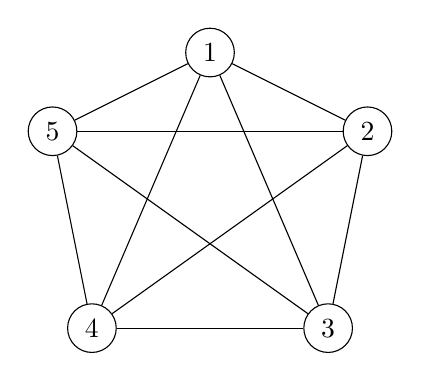
\begin{tikzpicture}[scale=1]
                % Déclaration des sommets avec des entiers pour K5
                \node[draw, circle] (1) at (0, 3.5) {1};
                \node[draw, circle] (2) at (2, 2.5) {2};
                \node[draw, circle] (3) at (1.5, 0) {3};
                \node[draw, circle] (4) at (-1.5, 0) {4};
                \node[draw, circle] (5) at (-2, 2.5) {5};

                % Ajout des arêtes pour K5 (chaque sommet est connecté aux autres)
                \draw (1) -- (2);
                \draw (1) -- (3);
                \draw (1) -- (4);
                \draw (1) -- (5);
                \draw (2) -- (3);
                \draw (2) -- (4);
                \draw (2) -- (5);
                \draw (3) -- (4);
                \draw (3) -- (5);
                \draw (4) -- (5);
            \end{tikzpicture}
            \caption{Graphe complet \( K_5 \)}
            \label{fig:K5-entiers}
        \end{minipage}
      \end{figure}
\end{example}

\begin{definition}[Bipartisme]
    Un graphe $G = (X,E)$ est dit biparti s'il existe une partition de $X$ en ensembles $X_1$ et $X_2$ non vides et disjoints tels que pour toute arrête $(x,y)$
    de $G$, $x$ et $y$ soient des ensembles différentes.
\end{definition}

\begin{remark}
    $G$ est dit $k$ parti, s'il existe une partition en $k$ ensembles de $X$ vérifiant la définition ci-dessus.
\end{remark}


\begin{example}
    Soit $G$ un graphe à 5 sommets biparti, alors :
    \begin{figure}[h]
        \centering
        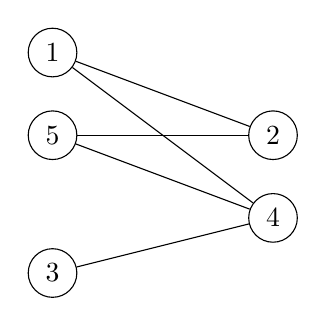
\begin{tikzpicture}[scale=0.7]
            \node[draw, circle] (1) at (-2, 4) {1};
            \node[draw, circle] (2) at (2, 2.5) {2};
            \node[draw, circle] (3) at (-2, 0) {3};
            \node[draw, circle] (4) at (2, 1) {4};
            \node[draw, circle] (5) at (-2, 2.5) {5};

            \draw (1) -- (2);
            \draw (1) -- (4);
            \draw (4) -- (3);
            \draw (4) -- (5);
            \draw (5) -- (2);
        \end{tikzpicture}
        \caption{Graphe biparti}
        \label{fig:K5-entiers}
    \end{figure}
\end{example}

\begin{example}[Graphe de Petersen]
    Sans doute l'un des graphes les plus connus en théorie des graphes, 
    le graphe de Pertersen en hommage à Julius Petersen qui l'étudia en 1898, possédant 10 sommets et 15 arrêtes possède 
    beaucoup de propriétés interressantes (notamment la connexité que nous verrons par la suite).
    Il est un contre-exemple pour beaucoup de propriétés et est très utile pour vérifier un algorithme en cours de développement ou une intuition. 
    \begin{figure}[h]
        \centering
        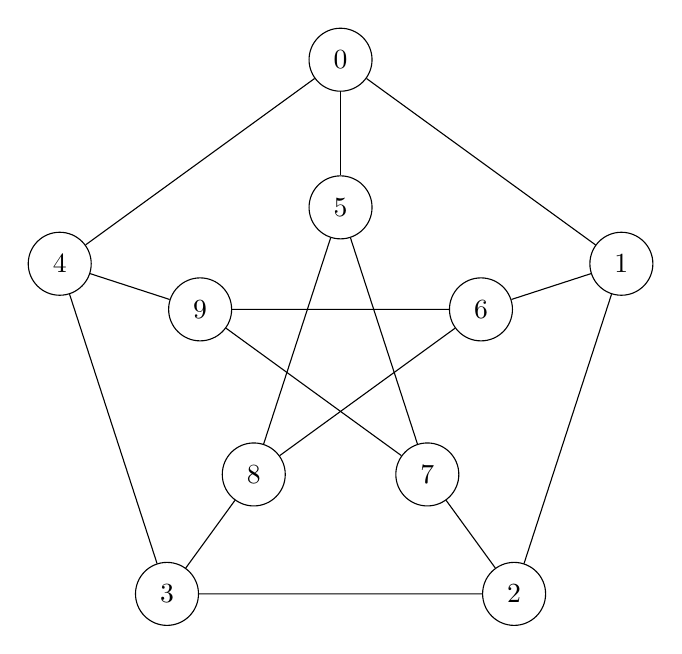
\begin{tikzpicture}[scale=1.25]

            % Coordonnées des sommets extérieurs
            \foreach \i in {0,1,2,3,4} {
                \node[circle, draw, minimum size=8mm] (a\i) at (90-\i*72:3) {\i};
            }
            
            % Coordonnées des sommets intérieurs
            \foreach \i in {5,6,7,8,9} {
                \node[circle, draw, minimum size=8mm] (b\i) at (90-\i*72:1.5) {\i};
            }
            
            % Arêtes du pentagone extérieur
            \foreach \i [count=\j from 1] in {0,1,2,3,4} {
                \pgfmathtruncatemacro{\nexti}{mod(\i+1,5)}
                \draw (a\i) -- (a\nexti);
            }
            
            % Arêtes du pentagone intérieur
            \foreach \i [count=\j from 1] in {5,6,7,8,9} {
                \pgfmathtruncatemacro{\nexti}{mod(\i+2,5)+5}
                \draw (b\i) -- (b\nexti);
            }
            
            % Arêtes reliant les sommets intérieurs aux sommets extérieurs
            \foreach \i in {0,1,2,3,4} {
                \pgfmathtruncatemacro{\j}{\i+5}
                \draw (a\i) -- (b\j);
            }
            
            \end{tikzpicture}
            \caption{Graphe de Petersen}
            \label{fig:K5-entiers}
    \end{figure}
\end{example}


\subsubsection{Propriétés}

\begin{prop}
    Soit $G$ un graphe non orienté simple à $n$ sommets.
    \begin{itemize}
        \item Si $G$ est complet, il possède $m =\frac{n(n-1)}{2}$ arrêtes.
        \item $G$ vérifie donc toujours $ m \leq \frac{1}{2} n (n-1)$
        \item $\sum_{x \in X} d(x)$ est le nombre d'extrémités d'arrêtes, c'est aussi deux fois le nombre d'arrêtes.
        \item Il y a un nombre pair de sommets de degré impairs.
    \end{itemize}
\end{prop}


\subsubsection{Graphes partiels et sous-graphes}

\begin{definition}[Graphe partiel]
    Soit $G = (X,E)$ un graphe. Le graphe partiel $G' = (X,E')$ de $G$ est tel que $E' \subset E$.
    Autrement dit, le graphe partiel d'un graphe $G$ est le même graphe mais avec quelques arrêtes en moins.
\end{definition}

\begin{definition}[Sous-graphe]
    Soit $G = (X,E)$ un graphe. Le graphe $G' = (X',E')$ de $G$ est tel que $X' \subset X$ et $E' = \{(x,y) : x \in X', y \in X', (x,y) \in E\}$.
    Autrement dit, le sous-graphe d'un graphe $G$ est le même graphe mais avec quelques sommets en moins (et donc quelques arrêtes en moins aussi).
\end{definition}

\begin{definition}[$k$-clique]
    Soit $G$ un graphe. On appelle $k$-clique, $k \leq n$, un sous-graphe complet de $G$de taille $k$.
\end{definition}


\subsubsection{Chaines et Cycles d'un graphe non orienté}

\begin{definition}[Chaine]
    On appelle chaine de $G$ de longueur $n$ toute suite alternée de sommets et d'arrêtes de $G$ telle que :
        \[ c = (x_0, a_1, x_1, \dots, a_n, x_n), \text{  telle que } \forall i \in \llbracket 1, n \rrbracket, a_i = (x_{i-1}, x_i) \]
    Ici, $n$ représente le nombre d'arrêtes de la chaine. Dans le cas d'un graphe simple, on notera les chaines de la façon suivante :
        \[ c = (x_0, \dots, x_n) \quad \text{ou} \quad c = x_0 - x_1 - \dots - x_n \] 
\end{definition}

\begin{definition}[Accessibilité]
    Soit $G = (X,E)$ un graphe. On a :
    \begin{itemize}
        \item Soient $x$ et $y$ deux sommets de $G$. On dit que $y$ est accessible à partir de $x$ s'il existe une chaine joignant $x$ et $y$ dans $G$.
        \item $G$ est dit \textbf{connexe} ssi $ \forall x \in X, \forall y \in X$, $y$ est accessible à partir de $x$.
        \item L'accessibilité est un relation d'équivalence entre les sommets. 
        
        Ses classes d'équivalences sont les composantes connexes de $G$.
    \end{itemize}
\end{definition}

\begin{definition}[Chaîne Simple]
    Une chaine est \textbf{simple} si elle ne passe pas deux fois par le même arrête et elle est dite élémentaire si elle ne passe pas deux fois pas le même sommet.
    On remarquera facilement qu'une chaîne élémentaire est simple.
\end{definition}

\begin{definition}[Cycle]
    Un cycle de $G$ est une chaine simple dont le départ et l'arrivée sont le même sommet. Un cycle est donc de la forme :
        \[ c = x_0 - x_1 - \dots - x_{n-1} - x0 \] 
\end{definition}

\begin{theorem}[Propriétés des cycles et chaînes]
    Soit $G$ un graphe.
    \begin{itemize}
        \item Toute chaine élémentaire a une longueur inférieure à $n-1$
        \item Toute cycle élémentaire a une longueur inférieure à $n$
        \item De toute chaîne, on peut en extraire une chaîne élémentaire.
    \end{itemize}
\end{theorem}


\subsubsection{Chemins, circuits d'un graphe orienté et forte connexité}

On utilise la même définition de chemin et circuit. Seulement, si le graphe est simple, il sera inutile de préciser les arrêtes par lesquelles on passe.

\begin{definition}[Forte Connexité]
    Un graphe $G = (X,E)$ orienté est dit fortement connexe si pour tout somet $x$ et $y$ de $G$, $y$ est accessible à partir de $x$.
\end{definition}


\begin{definition}[Arbre]
    On appelle arbre un graphe non orienté, connexe et sans cycle. Un graphe non orienté et sans cycle, i.e une union d'arbres et appelé \textbf{forêt}.
\end{definition}

\begin{theorem}[Caractérisation d'un arbre]
    Soit $T$ un graphe à $n$ sommets et $m$ arrêtes. $T$ est un arbre ssi :
    \begin{itemize}
        \item[\empty] $T$ est sans cycle et $m = n-1$ 
        \item[$\Longleftrightarrow$] $T$ est connexe et $m = n-1$
        \item[$\Longleftrightarrow$] $T$ est sans cycle et maximal au sens des arrêtes
        \item[$\Longleftrightarrow$] $T$ est connexe et minimal au sens des arrêtes 
        \item[$\Longleftrightarrow$] Deux sommets quelconques de $T$ sont reliés par un unique chemin.  
    \end{itemize}
\end{theorem}

% ==================================================================================================================================
% Représentation d'un graphe

\subsection{Représentations d'un graphe}

\subsubsection{Représentation par liste d'arrêtes}

\begin{definition}[Liste d'arrêtes]
    On appelle liste d'arrêtes de $G$ la liste des couples $(x,y)$ avec $x \in X$ et $y \in X$ tels que $(x,y) \in E$
\end{definition}


\begin{example} Représentations par liste d'arrêtes/d'arcs
    \begin{itemize}
        \item Le graphe orienté $G_1$ est représenté par la liste d'arcs :
            \[ [[1, 5], [2, 1], [2, 4], [3, 2], [4, 3], [5, 2], [5, 4]] \]
        \item Le multigraphe non orienté $G_2$ est représente par la liste d'arrêtes :
            \[  [[1, 2], [1, 5], [1, 5], [2, 1], [2, 4], [2, 4], [2, 3], [3, 2], [3, 3], [3, 4], [4, 2], [4, 2], [4, 3], [4, 5], [5, 1], [5, 1], [5, 4]] \] 
    \end{itemize}
    \begin{figure}[h]
        \centering
        \begin{minipage}{0.45\textwidth}  % Première image dans 45% de la largeur de la page
            \centering
            \begin{tikzpicture}[->,>=stealth',shorten >=1pt,auto,node distance=2cm,thick,scale=0.7]
                % Déclaration des sommets avec des entiers pour K4
                \node[draw, circle] (1) at (-1, 2) {1};
                \node[draw, circle] (2) at (1, 2) {2};
                \node[draw, circle] (3) at (2.5, 1) {3};
                \node[draw, circle] (4) at (1, 0) {4};
                \node[draw, circle] (5) at (-1, 0) {5};
            
                % Ajout des arêtes pour K4 (chaque sommet est connecté aux autres)
                \draw[->] (2) -- (1);
                \draw[->] (1) -- (5);
                \draw[->] (5) -- (4);
                \draw[->] (5) -- (2);
                \draw[->] (2) -- (4);
                \draw[->] (4) -- (3);
                \draw[->] (3) -- (2);
              \end{tikzpicture}
              \caption{Graphe Orienté $G_1$}
              \label{fig:K4-entiers}
        \end{minipage}
        \hfill % Ajoute de l'espace flexible entre les deux images
        \begin{minipage} {0.45\textwidth}  % Deuxième image dans 45% de la largeur de la page
            \centering
            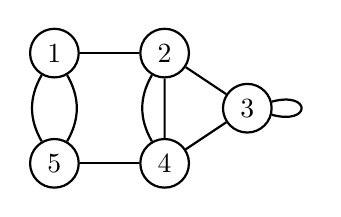
\begin{tikzpicture}[thick, scale=0.7]
                % Déclaration des sommets avec des entiers pour K5
                \node[draw, circle] (1) at (-1, 2) {1};
                \node[draw, circle] (2) at (1, 2) {2};
                \node[draw, circle] (3) at (2.5, 1) {3};
                \node[draw, circle] (4) at (1, 0) {4};
                \node[draw, circle] (5) at (-1, 0) {5};

                % Ajout des arêtes pour K5 (chaque sommet est connecté aux autres)
                \draw[bend left] (1) to (5);
                \draw[bend left] (5) to (1);
                \draw (5) -- (4);
                \draw (1) -- (2);
                \draw[bend right] (2) to (4);
                \draw (4) -- (2);
                \draw (4) -- (3);
                \draw (3) -- (2);
                \draw[loop right, -] (3) to ();
            \end{tikzpicture}
            \caption{Multigraphe non orienté $G_2$}
            \label{fig:K5-entiers}
        \end{minipage}
      \end{figure}
\end{example}

\subsubsection{Représentation Matricielle}

\begin{definition}[Matrice d'adjascence]
    On appelle matrice d'adjascence d'un graphe $G$ la matrice $A = (a_{ij})$ telle que 
    $\forall (i,j) \in X \times X$, on ait :
    \begin{itemize}
        \item Si $G$ est non orienté, $a_{ij}$ est égal à $1$ si $(i,j) \in E$ et $0$ sinon. La mrtice est donc symétrique.
        \item Si $G$ est orienté, $a_{ij}$ est égal à $1$ si $(i,j) \in E$
        \item Dans le cas d'un multigraphe, le coefficient $a_{ij}$ de la matrice d'adjascence de $G$ représente le nombre d'arrêtes entre les sommets $i$ et $j$ de $G$.
                Les coefficients diagonaux de la matrice représentent donc les boucles de $G$.
    \end{itemize}
\end{definition}


\begin{prop}
    Soit $G$ un graphe non orienté, et $A$ sa matrice d'adjascence.
    \begin{itemize}
        \item Puisque $G$ est non orienté, alors $A \in \mathcal{S}_n(\N)$ i.e $A$ est symétrique.
        \item La somme des éléments de la ligne $i$ est dégale à $d^-(i)$
        \item La somme des éléments de la colonne $i$ esy égale à $d^+(i)$
    \end{itemize}
\end{prop}

\begin{example}[Matrices d'adjascences]
    \begin{multicols}{2}
        La matrice d'adjascence de $G_1$ :
        \[ M_1 = 
        \begin{pmatrix}
            0 & 0 & 0 & 0 & 1 \\
            1 & 0 & 0 & 1 & 0 \\
            0 & 1 & 0 & 0 & 0 \\
            0 & 0 & 1 & 0 & 0 \\
            0 & 1 & 0 & 1 & 0 
        \end{pmatrix} \] 
        \vfill % Remplit l'espace verticalement pour ajuster la hauteur
        \columnbreak % Barre de séparation entre des deux colonnes
        La matrice d'adjascence de $G_2$ :
        \[ M_2 = 
        \begin{pmatrix}
            0 & 1 & 0 & 0 & 2 \\
            1 & 0 & 1 & 2 & 0 \\
            0 & 1 & 1 & 1 & 0 \\
            0 & 2 & 1 & 1 & 1 \\
            2 & 0 & 0 & 1 & 0
        \end{pmatrix} \] 
    \end{multicols}
\end{example}

\begin{remark}[Algèbre Linéaire]
    Comme dans toutes les représentations matricielles de concepts (que ce soit des applications ou des graphes),
    elles nous permettent d'invoquer facilement tous les résultats d'algèbre linéaires tels que la réduction,
    les noyaux, rangs, la composition...tout en préservant les propriétés des objets étudiés.
\end{remark}

\begin{prop}
    Soit $A^k, k \in \N$ où $A$ est la matrice d'adjascence d'un graphe $G$.
    Alors le coefficient d'indice $(x,y)$ de $A^k$ est le nomdre de chemins de longueur $k$ entre les sommets $x$ et $y$.
\end{prop}

\begin{remark}
    Toutefois, la représentation matricielle d'un graphe n'est pas optimale pour parcourir ces derniers puisque, ainsi, 
    les algorithmes de parcours auront forcément une complexité temporielle/spatiale en $\Theta(n^2)$.
\end{remark}

\subsubsection{Représentation par liste d'adjascence}

\begin{definition}[Liste d'adjascence]
    La liste d'adjascence d'un graphe $G$ est un vecteur $L$ indexé par $X$ tel que pour tout sommet $x \in X$,
    $L[x]$ est la liste des successeurs de $x$ dans $G$.
\end{definition}

\begin{example}
    Reprenons les graphes $G_1$ et $G_2$ représentés plus haut. On a alors :
    \begin{itemize}
        \item $G_1 = \{1 : [5],2 : [1,4],3 : [2],4 : [3],5 : [2,4]\}$
        \item $ G_1 = \{1 : [2,5,5],2 : [1,3,4,4],3 : [2,3,4],4 : [2,2,3,5],5 : [1,1,4]\}$
    \end{itemize}
\end{example}

\begin{remark}
    On remarque vite que cette représentation sera plus optinale. Premièrement, le parcours d'un graphe se fera en $\Theta(n)$ 
    et pour chaque sommet, on obtiendra sa liste de successeurs en $\Theta(1)$, si on représente une liste d'adjascence sous forme de dictionnaire en Python.
\end{remark}

\begin{prop}
    Pour chaque graphe à $n$ sommets et $m$ arcs, l'espace mémoire utilisé est un $\Theta(n+m) = \Theta (\max \{n,m\})$.
\end{prop}


\subsection{Parcours d'un graphe}

\subsubsection{Parcours en profondeur (Depth First Search)}

Le parcours en profondeur est à voir comme le parcours d'un chien fou dans un labyrinthe.
Celui-ci va partir dans un couloir et à chaque intersection va aller sur le chemin le plus proche jusqu'à arriver à une impasse.
A chaque impasse, il va revenir sur ses pas pour parcourir les autre chemins les plus proches. Le tout jusqu'à parcourir tout le labyrinthe.

Ainsi, cet algorithme de parcours se concevra de manière récurisive où chaque appel récurisif représentera l'envoi du chien fou dans un chemin (ici une arrête).
D'où l'algorithme suivant :

\lstset{
    basicstyle=\ttfamily\small,
    commentstyle=\color{green},
    keywordstyle=\color{blue},
    numbers=left,
    stepnumber=1,
    frame=single,
    breaklines=true
}
\begin{lstlisting}
Visite est initialise a l'ensemble vide 
Profond (G,x) :
    x est visite
    {Traiter x en premiere visite}
    Pour chaque voisin y de x faire :
        Si y n'est pas visite, alors :
            Profond(G,y)
        {Sinon on detecte une revisite de y}
    {Traiter x en derniere visite}
\end{lstlisting}


A partir du parcours en profondeur, on peut définir un ordre de parcours qui sera représenté par une liste de sommets.
Nous avons donc l'ordre de parcours en première visite (que l'on mettra à jour ligne 3 de l'algorithme)
et l'ordre de parcours en derniere visite (mis à jour ligne 9).

Pour un graphe $G$ non connexe ou non fortement connexe, le parcours en profondeur lancé à partir d'un unique sommet ne 
permettra pas d'accéder à tous ses sommets. D'où le parcours dit généralisé où l'on itère sur tous les sommets de $G$ et s'il n'est 
pas visité, on lance un parcours en profondeur à partir de celui-ci.

Ainsi, le parcours en profondeur généralisé d'un graphe $G$ permet de définir une arborescence de parcours.

\begin{definition}[Arborescence de parcours - profondeur]
    L'arborescence de parcours en profondeur de $G$ à partir d'un sommet $x \in X$ est une arbre $A$ enraciné en $x$, orienté, tel qu'il existe un arc $(x,y)$ dans $A$ 
    ssi l'appel à profond(G,x) a engendré récurisivement un appel à profond(G,y).
\end{definition}

A la fin d'un parcours en profondeur généralisé d'un graphe $G$, on obtient donc une forêt de visite contenant tous les sommets de $G$, i.e tous les sommets de $G$ ont étés visités.

\subsubsection{Parcours en largeur (Breadth First Search)}

Le parcours en largeur est fondamentalement différent de celui en profondeur. 
Tout d'abord, nous pouvons reprendre la comparaison avec le parcours d'un labyrinthe par un chien. 
Ici, notre chien sera vieux et plus malin. Pour chaque intersection (sommet), il va se rappeler de tous les chemins
à proximité (sommets voisins). Il se dirigera donc vers l'intersection (sommet) la plus ancienne qu'il ait retenue pour ensuite lister toutes
ses voisinnes, et ainsi de suite.
Pour ne pas tourner en rond, à chaque fois qu'il voit une intersection (sommet) voisinne, il vérifie qu'il ne l'aie pas visitée avant de la retenir.
Le vieux chien d'arrête donc dès qu'il n'a plus d'intersection (sommet) à visiter en mémoire.

On peut donc implémenter cette algorithme de façons itérative où un ensemble représentera les sommets déjà visités
et une file d'attente les sommets à visiter. Le premier sommet de file sera donc le prochain sommet à visiter.

\begin{lstlisting}
Visite est initilise a l'ensemble vide 
Largeur(G,x):
    F = [X]
    Visite[x] = vrai 
    Tant que F n'est pas vide, faire :
        Considerer la tete y de F et l'enlever de F 
        {Traiter y}
        Pour chaque successeur z de y, faire :
            Si z n'est pas visite, alors 
                z est visite 
                ajouter z a la fin de la file F 
\end{lstlisting}

De même que le parcours en profondeur, on peut définir un ordre de parcours, en première ou derniere visite.
Comme le parcours en profondeur, parfois nous auront besoin de lancer un parcours généralisé à tout le graphe pour parcourir tous ses sommets.

\begin{definition}[Arborescence de parcours - largeur]
    L’arborescence de parcours en largeur de $G$ à partir du sommet x est un arbre $A$  enraciné en x, orienté 
    tel qu’il existe un arc $(y,z)$ dans $A$ ssi le traitement de $y$ ajoute le sommet $z$ dans la liste d’attente $F$.
\end{definition}

La tableau Visite est intilisé en $\Theta(n)$. Le parcours est appelé exactement une seule fois pour chaque sommet $x$ de $G$ 
et a pour complexité $\Theta(1)$ pour le traitement de $x$ et $\Theta(d(x))$ pour l'exploration des successeurs de $x$.
La complexité des deux parcours est donc : 
\begin{align*}
    C(n) &= \Theta(n) + \sum_{x=1}^{n} (d(x) + \Theta(1)) \\ 
            &= \Theta(N) +  \sum_{x=1}^{n} d(x) \\
            &= \Theta(n) + \Theta(m) \\
            &= \Theta (\max \{n,m\})
\end{align*}


Maintenant que l'on sait parcourir un graphe, on peut étudier ses propriétés plus facilement.
Voici quelques exemples d'applications interressantes :

\subsubsection{Classification des arcs}

Une fois le parcours réalisé, on remarque que la forêt de parcours est composée de différents types d'arcs.
Soit $(x,y)$ un arc de $G$, il est dit...
\begin{itemize}
    \item \textbf{Couvrant} ssi $(x,y)$ est un arbre de la forêt de visite.
    \item \textbf{En avant} ssi il existe un chemin de $x$ à $y$ dans la forêt de visite de $G$.
    \item \textbf{En arrière} ssi il est chemin de $y$ à $x$ dans la forêt de visite.
    \item \textbf{Transverse} ssi ce n'est pas un arc ci-dessus.
\end{itemize}
La présence de cycle dans un graphe se manifestera par un arc arrière dans l'arbre de visite et un arc avant peut être vu comme un raccourci dans $G$.
Notons que pour chaque parcours, certains arcs sont présents et d'autres non.

\subsubsection{Existence de chemins et connexité}

Les deux parcours d'un graphe à partir d'un sommet $x$ nous permettent de trouver tous les sommets accessibles à partir de $x$.
Donc on peut facilement adapter un algorithme pour déterminer s'il existe un chemin entre deux sommets $x$ et $y$ de $G$, et même en trouver.

Dans le cas d'un graphe \textbf{non orienté}, si le parcours à partir d'un sommet $x$ atteint tous les autres sommets $y$ de $G$, alors $G$ est connexe et réciproquement.


\vspace{3cm}


\begin{quote}
    \centering
    \emph{"A partir d'ici, vous ne vous perdez plus dans les labyrinthes."} Thierry Montaut
    \justify
\end{quote}


% ==================================================================================================================================
% Modélisation et Graphes

\section{Modélisation et Graphes}

\subsection{Chemins et circuits Eulérien}

\subsubsection{Les 7 ponts de Königsberg}

Le problème des 7 ponts de Königsberg consiste à savoir s'il est possible de déterminer une promenade passant par tous les 
ponts de la ville de Königsberg en passant une et une seule fois par chaque ponts de la ville et en revenant à son point de départ. 
Ce problème est sûrement le plus connu de l'histoire de la théorie des graphes et fut résolut par \textbf{Leonhard Euler} en 1735. 
Il explique que le problème n'est pas résoluble pour la ville de Königsberg et établit ainsi l'un des tout premiers théorèmes 
de théorie des graphes. 

La démonstration mathématique du théorème d'Euler ne fut énoncée qu'en 1873 par Carl Hierholzer. 

Des problèmes similaires existent tels que celui du facteur chinois qui cherche à effectuer sa tournée de distribution en 
passant une et une seule fois par chaque rue et en revenant à son point de départ (Mai-Ko-Kwan, 1962).


\begin{definition}[Graphe Eulérien/Circuit Eulérien]
    Soit $G = (X,E)$ un graphe non orienté, un circuit eulérien dans $G$ est un circuit passant une et une seule 
    fois par chaque arrête et revenant au sommet de départ. 

    Un graphe est dit eulérien ssi il possède un circuit eulérien. 
\end{definition}

\subsubsection{Théorème d'Euler}

\begin{theorem}[Théorème d'Euler]
    Soit $G$ un graphe non orienté \textbf{connexe}. 
    \begin{itemize}
        \item $G$ admet un circuit eulérien ssi tous ses sommets sont de degré pair. 
        \item $G$ admet un circuit eulérien ssi tous ses sommets ont un degré pair seuf deux sommets $a$ et $b$
        alors, tous les circuits eulériens de $G$ on a/b comme sommet de départ et b/a comme sommet d'arrivée.  
    \end{itemize}
\end{theorem}

\subsubsection{Algorithme de recherche de circuits eulérien}

L'objectif de l'algorithme est de construire un circuit eulérien dans un graphe en considérant un graphe partiel
du graphe initial. A chaque étape, on cherche un chemin maximal partant du premier sommet non saturé du chemin précédent
et qui revient à ce sommet. Puisque il existe un nombre pair de sommets de degré impair il existe un tel sommet à chaque itération. 

A la fin de l'algorithme on "recolle" tous les chemins bout à bout en un seul chemin simple non extensible passant par toutes 
les arrêtes, créant ainsi un circuit eulérien. 

L'idée est de créer une "copie" du graphe et, lors de la création d'un chemin à une certaine étape, d'enlever les arrêtes concernées
par le chemin pour éviter qu'elles ne soient réutilisées. 


\subsection{Problème de coloration}

Les problèmes de colorations de graphes, en plus d'êtres difficiles à résoudre, sont, cependant, très facile à imaginer. 
L'exemple le plus typique est celui de la coloration d'une carte géographique. En essayant de colorier une carte de l'Europe
d'une telle façon que deux pays limitrophes n'aient pas la même couleur, on s'apperçoit vite que cela peut être compliqué, 
surtout si on essaye d'utiliser le moins de couleurs possibles.

C'est exactement ce que modélisent les problèmes de coloration de graphes. On essaye d'attribuer à chaque sommet une couleur
de telle sorte que tous ses voisins n'aient pas la même couleur que lui en utilisant le moins de couleurs possibles. 

\begin{definition}[$k$-coloration]
    Soit $G$ un graphe non orienté. On dit que $G$ admet une $k$-coloration s'il existe $k$ couleurs différentes 
    telles que deux sommets adjacents de $G$ n'aient pas la même couleur. 
\end{definition}

\begin{prop}[Propriétés des colorations]
    \begin{itemize}
        \item Si $G$ est $k$-parti alors $G$ est $k$-colorable. 
        \item Si $G$ est un graphe complet de taille $n$ alors $G$ ne peut pas être colorié avec moins de $n$ couleurs. 
        \item Si $G$ admet une $k$-clique, alors $G$ ne peut pas être colorié avec moins de $k$ couleurs.
    \end{itemize}
\end{prop}

\begin{definition}[Nombre Chromatique]
    On appelle nombre chromatique $\gamma(G) = k$ d'un graphe $G$ le plus petit entier positif tel que $G$ admette une $k$-coloration.
\end{definition}

\subsubsection{Coloration Naïve}

Premier algorithme de coloration de graphe, il est très facile à comprendre et à mettre en oeuvre mais 
est particulièrement gourmand en couleurs. 

L'idée est de parcourir le graphe dans l'ordre naturel des sommets et d'attribuer à chaque sommet 
la plus petite couleur non attribuée à ses voisins. 

Il faut donc une fonction permettant de parcourir le graphe et une autre déterminant 
la plus petite couleur non attribuée aux voisins d'un sommet. 
La coloration est représentée par un dictionnaire dont les clés sont les sommets 
du graphe et les valeurs, les couleurs attibuées aux sommets. 

C'est un algorithme très peut coûteux d'une complexité en $\Theta(m)$ mais pas très optimal, 
puisque en fonction de l'ordre de visite des sommets, le nombre de couleurs utilisées peut 
varier. Il est très peu efficace pour de gros graphes. 

\subsubsection{Coloration Gloutonne}

Prenez vos crayons de couleurs préférés et essayer de colorier un graphe. 
Vous alez d'abord colorier tous les sommets possibles avec un certaine couleurs. 
Puis une fois que vous ne pouvez plus colorier de sommets de cette couleur tel qu'aucun 
de ses voisins n'est déjà colorié vous prenez une autre couleur et refaites de même. 
Le tout jusqu'à ce que tous les commets soient coloriés. 

C'est le principe de l'algorithme de coloration Gloutonne. A chaque étape, on choisit une 
couleur et on essaye de colorier le maximum de sommets non adjacents avec cette même couleur. 
Pour cela, nous allons considérer le noyau d'une graphe. 

\begin{definition}[Noyau]
    Soit $G = (X,E)$ un graphe. On appelle noyau de G un ensemble maximal de sommets 
    non adjacents deux à deux. 
\end{definition}

On va donc déterminer tous les noyaux de G en détruisant petit à petit le graphe. 
Et, pour chaque noyau de trouvé, on colorie tous les sommets du noyau avec la même couleur. 


\subsection{Ordonnancement}

Ici, un graphe représente un système de dépendances entre différentes tâches d'un même projet. 
Chaque sommet repésente une tâche à effectuer et une arrête d'un sommet $x$ vers un sommet $y$ indique que 
la tâche $y$ doit attendre que la tâche $x$ est terminée avant d'être commencée. 

On va donc essayer d'établir un graphe d'ordonnancement des tâches visant à indiquer dans quel ordre les différentes 
tâche devront être traitées. Mais pour cela, il faut définir certaines conditions sur le graphe de dépendances. 

\begin{proposition}
    Soit $G = (X,E)$ un graphe. 
    \begin{itemize}
        \item Si G est sans circuit, alors tous ses sous-graphes sont sans circuits. 
        \item Si G est sans circuit, le graphe inverse de G est sans circuit. 
        \item G est sans circuit ssi tous ses chemins sont élémentaires. 
    \end{itemize}
\end{proposition}

\begin{definition}[Sommets remarquables d'un graphe sans circuit]
    Soit $G = (X,E)$ un graphe orienté sans circuit. On définit :
    \begin{itemize}
        \item une \textbf{source} comme étant un sommet dont le degré entrant est nul. 
        \item un \textbf{puit} comme étant un sommet dont le degré sortant est nul. 
    \end{itemize}
\end{definition}

\begin{theorem}[Fondamental de l'ordonnancement]
    Tou graphe sans circuit possède une source et un puit. 
\end{theorem}

\subsubsection{Tri Topologique - Ordonnancement séquentiel}

\begin{definition}[Tri Topologique]
    On appelle tri topologique d'un graphe orienté une numérotation des des sommets respectant l'ordre des arcs. 
\end{definition}

\begin{theorem}[Condition d'existence d'un tri topologique]
    Soit $G = (X,E)$ un graphe orienté. G admet un tri topologique ssi il est sans circuit. 
\end{theorem}

Le principe de l'algorithme de tri topologique est \textbf{itératif}. 
Il repose sur le fait que tout graphe sans circuit \textbf{possède une source}. 
On va donc, à chaque étape, chercher une source du graphe et l'insérer dans notre tri topologique. 
L'étape suivante, on \textbf{considère le sous-graphe} du graphe initial auquel on a enlevé la source et tous les 
arcs sortants. 

Si on ne souhaite pas détruire le graphe, on va considérer les \textbf{degrés entrants} de chaque sommets dans un \textbf{dictionnaire} des degrés.

\lstset{
    basicstyle=\ttfamily\small,
    commentstyle=\color{green},
    keywordstyle=\color{blue},
    numbers=left,
    stepnumber=1,
    frame=single,
    breaklines=true
}
\begin{lstlisting}
S:=[];T:=[];
Pour x de 1 a n faire
    Degre[x]:=d^-(x) dans G;
    Si Degre[x]=0 alors ajouter x a S;
{S contient alors toutes les sources de G}

Tant que S<>[] faire
    x:=enleverTete(S);
    ajouterFin(x,T)

    {Mettre a jour les degres}
    Pour chaque successeur y de x dans G faire
        Degre[y]:=Degre[y]-1;
        si Degre[y] = 0 alors ajouterFin(y,S)
\end{lstlisting}

L'algorithme repose donc sur un \textbf{parcours en largeur}. On utilise une \textbf{file} pour stocker les 
sommets de degré entrant nul (i.e les sources). A chaque itération, on décrémente tous les degrés entrants des fils de la source, 
puis on ajoute la source à la liste représentant le tri topologique. 


\subsubsection{Tri par Niveaux - Ordonnancement en parallèle}

Ici, comparé à un tri topologique, on va construire un graphe d'ordonnancement en considérant que l'on peut effectuer plusieurs 
tâches en même temps. 

\begin{definition}[Tri par niveaux]
    Soit $G = (X,E)$ un graphe orienté, sans circuit. 
    Un tri par niveaux de G est une partition de G en niveaux tels que pour chaque sommet d'un même niveaux, 
    son exécution n'est pas dépendante d'un sommet du même niveau ou d'un niveau suivant. 
\end{definition}

L'algorithme est sensiblement le même que le tri topologique. Il suffit juste de l'adapter 
pour \textbf{traiter en même temps} toutes les sources de G. 
On définit alors \textbf{deux listes N1 et N2} représentant deux niveaux successifs. 
Le traitement des sources de N1 permet de déterminer les sources de N2. 

\begin{lstlisting}
N1:=[];T:=[];
Pour x de 1 a n faire
    Degre[x]:=d^-(x) dans G;
    Si Degre[x]=0 alors ajouter x a N1;
{S contient alors toutes les sources de G}

tant que N1<>[] faire
    ajouterFin(N1,T);
    N2:=[];
    pour tout x dans N1 faire
        {Mettre a jour les degres des successeurs de x et calcul}
        Pour chaque successeur y de x dans G faire
        Degre[y]:=Degre[y]-1;
        si Degre[y] = 0 alors ajouterFin(y,N2)
    N1:=N2;
\end{lstlisting}


\subsection{Arbre couvrant de poids minimum}

Ici, on considère un \textbf{graphe non orienté valué }pour lequel on va chercher un sous-arbre couvrant de poids minimal. 
Cela peut éventuellement modéliser le problème d'un électricien qui doit relier différentes pièces par un câble 
et cherche à utiliser le moins de câble électrique possible. 

\begin{definition}[Valuation]
    Soit $G = (X,E)$ un graphe non orienté. Une valuation est une fonction 
    \[ p : E \longrightarrow \R \] 
    qui, à chaque arrête lui associe une valeur appelée poids. 

    Un graphe muni qu'un valuation est appelé graphe valué. 
\end{definition}

Pour \textbf{représenter} un graphe valué, nous allons toujours utiliser une liste d'adjacence. 
Mais nous allons rajouter une matrice de poids représentée par un dictionnaire dont les clés sont les arrêtes (couple)
et la valeur, le poids de l'arrête correspondante. 

On pourra aussi représenter un graphe valué par une liste d'arrêtes composée de triplet représentant les deux sommets de l'extrémité 
de l'arrête et le poids de l'arrête. 

\begin{definition}[Arbres couvrant]
    Soit $G = (X,E)$ un arbre graphe non orienté valué. 
    Un arbre couvrant de G est un graphe partiel de G, $A = (X,E')$ qui soit un arbre. 
\end{definition}

\begin{theorem}[Condition d'existence]
    Soit $G = (X,E)$ un graphe non orienté valué. G admet un arbre couvrant ssi il est connexe. 
\end{theorem}


\subsubsection{Algorithme de Kruskal}

L'algorithme de Kruskal construit de \textbf{manière itérative} un arbre couvrant de poids minimal. 
Pour cela, on va considérer les arrêtes par ordre de poids croissant. A chaque itération, on va essayer d'ajouter 
\textbf{la plus petite arrête ne créant pas de cycle} à l'arbre couvrant. 

On s'arrête lorsque l'on a ajouté $n-1$ arrêtes. 

\begin{remark} (Condition d'arrêt et vérification)
    \begin{itemize}
        \item A chaque itération, il faut vérifier que le graphe construit de possède pas de cycle, il faut donc effectuer 
            un \textbf{parcours en largeur}. 
        \item Si à une itération, on ne trouve pas d'arrête qui convienne, c'est que le graphe n'était initialement pas connexe. 
    \end{itemize}
\end{remark}

\subsubsection{Algorithme de Prim}

L'algorithme de Prim cherche, contrairement à Kruskal, à \textbf{conserver la connexité à moindre coût}. 

On va donc considérer deux ensembles :
\begin{itemize}
    \item C : l'ensemble des arrêtes de T (arbre couvrant)
    \item M : le complémentaire de C dans X 
\end{itemize}

A chaque étape, on va donc chercher une arrête \textbf{joignant un sommet de C à un sommet de M dans G. }
Un arrête joignant deux composantes connexe ne pouvant pas créer de cycle, le graphe T reste bien un arbre. 

On s'arrête lorsque \textbf{T contient tous les sommets de G}. 

% \subsubsection{Implémentation}

\begin{comment}
    \begin{lstlisting}
    {Initialisations}
    T:=[];m:=0;
    M:=[];
    connexe:=vrai
    Pour i de 1 à n faire
        DIST[i]:=p(x,i); {S’il n’y a pas d’arete (x,i) p(x,i) renv
        MIN[i]:=x
        Si i<>x alors ajouterfin(i,M)

    Tant que connexe et m<n-1 faire
        {(1) chercher l’arête (y,z) de poids minimal telle que y soit dans C et z dans M}
        z:=min(DIST); {pas la valeur mais l’indice}
        si z=0 {toutes les valeurs de DIST sont infinies} alors c
        Debut
        enlever(z,M);
        y:=MIN[z];
        u:=(yz);
        Ajouterfin(u,T);
        m:=m+1;
    \end{lstlisting}
\end{comment}


\subsection{Plus courts chemins dans un graphe valué}

On considère ici un \textbf{graphe orienté valué}. 
L'objectif est de trouver un chemins entre deux sommets $x$ et $y$ dans G de poids minimal. 
On retrouve le même problème pour le routage de paquets dans un réseau. En effet, lors de l'établissement 
des tables de routage, on va chercher le chemin le plus court (au sens de la durée de transfert) entre deux noeuds. 


\begin{definition}[Cycle Absorbant]
    Dans le cas d'un graphe orienté, valué à \textbf{poids négatifs}, on appelle cycle absorbant 
    un cycle de coût total négatif. 
\end{definition}

\begin{remark}
    Le passage par un cycle absorbant dans un tel graphe fait diminuer le coût du chemin de poids minimal. 
    On comprend alors vite qu'un graphe avec un circuit absorbant ne possède pas de chemin de poids minimal. 
\end{remark}

\begin{theorem}[Condition d'existence]
    Soit $G = (X,E)$ un grapge orienté valué. Soient $x$ et $y$ deux sommets de G. 
    Alors il existe un chemin de poids minimal entre $x$ et $y$ ssi 
    \begin{itemize}
        \item $y$ est accessible à partir de $x$ 
        \item G ne possède pas de circuit absorbant
    \end{itemize}
\end{theorem}


\subsubsection{Algorithme de Dijkstra}

L'algorithme de Dijkstra 1 se base sur un \textbf{parcours en largeur} du graphe. 
On cherche tous les plus courts chemins d'un sommet s vers les autres sommets du graphe. 
Pour cela on dispose d'un \textbf{dictionnaire des poids}, et d'un \textbf{dictionnaire des pères}. 


A l'initialisation, on commence par parcourir tous les sommets du graphe à la recherche d'arrêtes partant de s. 
On va construire pas à pas un plus court chemin vers chaque sommet. A chaque étape, on considère tous les "nouveaux"
chemins vers les sommets du voisinnage du sommet traité. Si on trouve un chemin plus court, on remplace le chemin actuel et on remet le sommet dans la file. 
Dans le cas contraire, on ne fait rien. 

\begin{lstlisting}
M:={s};
{Initialisation}
Pour i de 1 a n faire
    Si (s,i) est une arete alors
        D[i]:=cout(s,i);
        P[i]:=s;
        ajouter(i,M);
    Sinon D[i]:=infini;

{Algorithme}
Tant que M<>{} faire
    x:=enleveTete(M);
    Pour tout successeur y de x faire
        d:=D[x]+cout(x,y);
        si d<D[y] alors
            D[y]:=d;
            P[y]:=x;
            ajouter(y,M)
\end{lstlisting}

L'algorithme de Dijkstra possède quand même quelques inconvénients. 
Un même sommet peut se retrouver plusieurs fois dans la file et on visite donc tous ses voisins plusieurs fois. 
Dans le cas \textbf{d'arrêtes à poids tous positifs}, on peut éviter tous ces parcours inutiles choisissant à chaque étape le sommet
dont le chemin depuis s est de coût minimal.

\subsubsection{Dijkstra Opt}

A chaque fois que l'on récupérer un sommet dans la file, on va \textbf{récupérer le sommet de poids minimal.} 
Pour cela, on va \textbf{garder la file triée selon le poids des sommets}. Il faut donc implémenter un fonction 
\texttt{insere} qui ajoute un sommet dans la file en fonction de son degré d'accessibilité. 

\begin{lstlisting}
{Initialisations}
M:={};
Pour i de 1 a n faire
    Si (s,i) est une arete alors
        D[i]:=cout(s,i);
        P[i]:=s;    
        ajouter(i,M);
    Sinon D[i]:=infini;

{Algorithme}
Tant que M<>{} faire
    x:=choisir_min(M,d);
    enlever(x,M);
    Pour tout successeur y de x faire
        Si y est dans M alors
            d:=D[x]+cout(x,y);
            si d<D[y] alors
                D[y]:=d;
                P[y]:=x;
                ajouter(y,M)
\end{lstlisting}

La \textbf{complexité} de l'algorithme de Dijkstra est donc en $$ \boxed{ \Theta(n^2) + \Theta(m) = \Theta(n^2) }$$

\subsubsection{Algorithme de Floyd}

Cet algorithme permet de calculer \textbf{tous les plus courts chemins} de tous les sommets vers tous les autres. 
Il a un \textbf{complexité} en $\Theta(n^3)$, donc il reste très efficace. 

L'algorithme repose sur une \textbf{idée itérative}. On commence donc par calculer tous les plus courts chemins de i vers j (deux voisins)
sans intermédiaires. 
Puis on calcule tous les plus courts chemins avec \textbf{un intermédiaire.}
$$ \dots$$ 
Arrivé à la n-ième itération, on a tous les plus courts chemins du graphe. 

Par \textbf{récurence}, pour passer de l'étape k à l'étape k+1 :
    \[ \forall (i,j) \in \{1,n\}^2, \quad d = pcc[(i,k)] + pcc[(k,j)] \] 
    \[ \text{si } d < pcc[(i,j)]: \] 
    \[ \quad pcc[(i,j)] = d \] 

On utilise une \textbf{matrice de poids} (pcc) et un \textbf{dictionnaire des pères} P. 


\subsubsection{Algorithme de Bellman (poids quelconques)}

Ici, on cherche les plus courts chemins d'un graphe orienté valué avec potentiellement des poids négatifs. 

L'idée est que si on connaît tous les plus courts chemins d'un sommet s vers tous les prédécesseurs d'un sommet y de G, 
alors, le plus court chemin de s vers y est : 
    \[ min (\{d_i + p_i, \quad  i \in \{i,n\}\})=: d_{i0} + p{i0}\]
et le prédécesseur de y dans le plus court chemin sera $x_{i0}$. 

A \textbf{l'initialisation}, on connaît tous les plus courts chemins de $s$ vers lui-même. 
On considère donc $G'$ le \textbf{sous-graphe} de G constitué des sommets dont one ne connaît pas encore de plus courts chemins. 
$G'$ est un sous-graphe d'un graphe sans cycle donc il admet toujours des \textbf{sources}. 
Une source de $G'$ est un sommets de $G'$ dont on connaît tous les prédécesseurs. On peut donc calculer son plus courts 
chemin comme vu précédement et il sort de $G'$. 

On va construire un \textbf{dictionnaire des distances} \texttt{Dist} et un \textbf{dictionnaire des pères} dans le plus court chemin \texttt{Pred}. 
Pour l'algorithme, on utilise un dictionnaire représentant le nombre de prédécesseurs inconnus d'un sommet. 

\begin{lstlisting}
# Sort de G'
Pour x dans G[y] faire :
    Deg[x] -= 1
    si Deg[x] == 0 :
        ajouter(x,S)
\end{lstlisting}

\begin{lstlisting}
# calcul du pcc vers y
{Soit H la liste des predecesseurs dans G}
Pour x dans H[y] faire :
    si Dist[x] + P[(x,y)] < D[y] faire :
        D[y] = Dist[x] + P[(x,y)]
        Pred[y] = x 
\end{lstlisting}

Pour représenter le graphe on a donc besoin :
\begin{itemize}
    \item La liste d'adjacence de G.
    \item Le dictionnaire des pères.
    \item La matrice de poids représentée par un dictionnaire. 
\end{itemize}

L'algorithme se base donc sur un \textbf{parcours en  largeur}, d'où :

\begin{lstlisting}
{Initialisation}
...
{Algorithme}
Tant que S<>[] faire :
    y = tete de S 
    # calcul pcc vers y 
    # y sort de G'
\end{lstlisting}

Cet algorithme a donc un \textbf{complexité} en : 
    $$ \Theta(m + n) $$



\chapter{Mots et Langages}
\minitoc % Ajoute le sommaire local ici

% ==================================================================================================================================
% Introduction 

Si on connaît plusieurs langages de programmation, on remarque que chaque langage, ou plutôt chaque paradigme de 
langage est spécialisé pour la résolution d'une carégorie dde problèmes. 
On pourrait se demander s'il est possible de créer un langage permettant de résoudre tous les problèmes. 
Pour cela, il nous faudrait d'abord être capable de définir formellement un langage, des mots, etc... 

% ==================================================================================================================================
% Alphabets et Mots 

\section{Alphabets et Mots}

\subsection{Premières Définitions}

Commençons tout d'abord par redéfinir correctement la notion d'alphabet et de mot. 

\begin{definition}[Alphabet]
    Un alphabet est simplement un ensemble fini, noté $\Sigma$.
    On nomme "lettre" ou "symbole" les éléments d'un alphabet.  
\end{definition}

\begin{example}
    Quelques exemples d'alphabets :
    \begin{itemize}
        \item $\Sigma = \{a,b\}$ 
        \item $\Sigma = \{a,b,\dots,\text{\%},\text{\$}\}$
    \end{itemize}
\end{example}

\begin{definition}[Mot]
    Un mot est une suite finie de lettres d'un alphabet. 
\end{definition}

\begin{proposition}
    Le mot vide est noté $\varepsilon$. On note l'ensemble des mots d'un alphabet $\Sigma^*$. 
\end{proposition}

\begin{definition}[Longueur d'un mot]
    On note $|w|$ la longueur d'un mot $w \in \Sigma^*$ qui correspond au nombre de lettres, avec répétition du mot $w$. 
\end{definition}

\begin{definition}[Egalité de mots]
    On dit que deux mots $u,v \in \Sigma^*$ son égaux ssi :
    \begin{itemize}
        \item $|v| = |u|$ 
        \item $\forall i \in \llbracket 1, |v| \rrbracket, \quad u[i] = v[i]$ où $u[i]$ est la ième lettre du mot $u$. 
    \end{itemize}
    \emph{Deux mot sont égaux ssi ils sont de même longueur et sont composés des mêmes lettres dans le même ordre.}
\end{definition}

\subsection{Opérations sur les mots}

Sur les mots, on ne définit qu'une seule opération, la \textbf{concaténation}. 

\begin{definition}[Concaténation]
    Soient $u,v \in \Sigma^*$ deux mots définis sur un même alphabet. On appelle la concaténation l'application :
    \[
        \begin{cases}
            \Sigma^* \times \Sigma^* \longrightarrow \Sigma^* \\ 
            (u,v) \longmapsto w = u.v
        \end{cases}
    \]
    Elle est définie telle que $ \forall u,v \in \Sigma^*$ de longueur $n,p \in \N$, on ait :
    \begin{itemize}
        \item $ |u.v| = |u| + |v| = n + p $
        \item $ \forall i \in \llbracket 1, n \rrbracket u.v[i] = u[i] $ et $ \forall i \in \llbracket 1,p \rrbracket, u.v[n+i] = v[i] $  
    \end{itemize}
    On parlera identiquement de concaténation ou de produit. 
\end{definition}

\begin{remark}
    Cette définition reprend bien la caractérisation de deux mots égaux. 
\end{remark}

\begin{proposition}[Propriétés de la concaténation]
    La concaténation est une application :
    \begin{itemize}
        \item \textbf{Associative : } $\forall u,v,w \in \Sigma^*, \quad w.(u.v) = (w.u).v$ 
        \item \textbf{Pas commutative} pour un alphabet de plus d'une lettre. 
        \item admet pour \textbf{élément neutre} le mot vide $\varepsilon$. 
    \end{itemize}
\end{proposition}

\subsection{Puissance d'un mot}

Une fois la concaténation définie pour un mot, on peut alors parler de puissance de mot. 
Définissons celle-ci par récurrence. 

\begin{definition}[Puissance d'un mot]
    Soit $\Sigma$ un alphabet et $ u \in \Sigma^*$, on a :
    \begin{itemize}
        \item $u^0 = \varepsilon $
        \item $u^1 = u$ 
        \item $ \forall n \in \N, u^{n+1} = u^n.u$ 
    \end{itemize}
\end{definition}

\begin{example}
    $(ba)^3 = bababa $
\end{example}

\begin{proposition}
    Soient $u \in \Sigma^*$ on peut appliquer les règles "connues" des puissances d'où : $$ \forall n,p \in \N, \quad  u^{n+p} = u^n . u^p = u^p . u^n $$ 
\end{proposition}

On remarque que l'on peut effectuer des simplifications sur les égalités de mots. 

\begin{prop}[Simplifications]
    L'ensemble $\Sigma^*$ est simplifiable à gauche et à droite. 
    \begin{itemize}
        \item $\forall u,v,w \in \Sigma^*, \quad u.w = v.w \Longrightarrow u = v $
        \item $\forall u,v,w \in \Sigma^*, \quad w.u = w.v \Longrightarrow u = v $
    \end{itemize}
\end{prop}

Ici, pas besoin d'inverse, la démonstration repose sur la définition de l'égalité entre deux mots. 

% ==================================================================================================================================
% Ordre

\newpage 

\section{Relations d'Ordre}

Dans l'alphabet dit "classique" on possède un ordre lexicographique des mots permettant de les classer 
en fonction de leurs lettres et de la position de leurs lettres. 
Ici, nous allons définir deux types de relations d'ordre sur les mots. 

Commençons par rappeler la définition de relation d'ordre. 

\begin{definition}[Relation d'Ordre]
    Soit $\lhd $ une relation sur un ensemble $E$. On dit que $\lhd$ est une \textbf{relation d'ordre} ssi 
    pour tout $x,y,z \in E$, $\lhd$ est :
    \begin{itemize}
        \item \textbf{Réflexive : } $ x \lhd x $ 
        \item \textbf{Anti-Symétrique : } $ x \lhd y \text{ et } y \lhd x \Longrightarrow x = y $ 
        \item \textbf{Transitive : } $x \lhd z \text{ et } z \lhd y \Longrightarrow x \lhd y $ 
    \end{itemize}
\end{definition}

\subsection{Ordre Préfixe}

Naturellement, on munit$ \Sigma^*$ d'un ordre préfixe permettant de classer les mots en fonction de leur préfixe. 
Cette relation peut être vue comme un forme d'inclusion de mots. 

\begin{definition}[Ordre Préfixe]
    Soient $u,w \in \Sigma^*$, on définit la relation d'ordre préfixe $\sqsubseteq$ telle que :
        \[ \boxed{u \sqsubseteq w \iff \exists v \in \Sigma^*, w = u.v} \] 
    Autrement dit, $u$ est un préfixe de $w$ ssi il existe un mot $v$ tel que $w$ soit composé de 
    la concaténation de $u$ et $v$. 
\end{definition}

\begin{remark}
    L'ordre préfixe ne nécessite pas de relation d'ordre directement sur l'alphabet $\Sigma$. 
\end{remark}

\begin{prop}[Ordre Préfixe et égalité]
    Soient $u,v \in \Sigma^*$ on a : 
        \[ u \sqsubseteq v \text{ et } v \sqsubseteq u \Longrightarrow u = v \] 
\end{prop}

\begin{quote}
    \begin{footnotesize}
        \begin{proof}
            Soient $u,v \in \Sigma^*$ tels que $ \exists x,y \in \Sigma^*$ tels que 
                \[ u = v.x \quad \text{ et } \quad v = u.y \] 
            On a alors que :
                \[
                    \begin{cases}
                        v = v.y.x \\ 
                        yx = \varepsilon 
                    \end{cases}
                    \; \Longrightarrow 
                    \begin{cases}
                        y = \varepsilon \\ 
                        x = \varepsilon 
                    \end{cases}
                    \; \Longrightarrow u = v 
                \]
        \end{proof}
    \end{footnotesize}
\end{quote}

\begin{remark}
    \textbf{Attention : } l'ordre préfixe est une relation d'ordre partielle. 
    Autrement dit, tous les éléments d'un même alphabet de sont pas comparables. 
\end{remark}

\subsection{Ordre Lexicographique}

\begin{definition}[Ordre Lexicographique]
    Soit $\Sigma$ un alphabet que l'on muni d'une relation d'ordre $\leqslant$. 
    L'ordre lexicographique $\leqslant$ est une relation d'ordre totale sur $\Sigma^*$. 
\end{definition}

\begin{remark}
    Ici, nous avons bien besoin de définir au préalable un ordre sur notre alphabet $\Sigma$. 
\end{remark}

\begin{prop}[Compatibilité]
    L'ordre lexicographique est compatible avec l'ordre préfixe. Plus formellement, 
        \[ \forall u,v \in \Sigma^*, \quad u \sqsubseteq v \Longrightarrow u \leqslant v \] 
\end{prop}



% ==================================================================================================================================
% Langage

\section{Langage}

Maintenant que nous sommes au clair sur la définition de lettre et de mot, on peut enfin définir l'objet 
principal de ce chapitre, les langages. 

\subsection{Definition}

\begin{definition}[Langage]
    Soit $\Sigma$ un alphabet, on appelle langage sur $\Sigma$ toute partie 
    de $\Sigma^*$. 
\end{definition}

\begin{remark}
    L'ensemble de tous les langages d'un alphabet $\Sigma$ est donc $\mathcal{P}(\Sigma^*)$, 
    l'ensemble de toutes les parties de $\Sigma^*$. 
\end{remark}

\begin{definition}[Complémentaire]
    Soit $L$ un langage sur $\Sigma$. On définit le complémentaire de $L$ dans $\Sigma^*$ le langage :
        \[ \overline{L} = \{w, \; w \not \in L\} \] 
\end{definition}

\subsection{Opérations}

De même que pour les alphabets et les mots, on peut définir des opérations sur les langages. 

\begin{definition}[Opérations sur les langages]
    Soit $\Sigma$ un alphabet et $L_1, L_2 \subseteq \Sigma^*$ deux langages de $\Sigma$. 
    On définit 4 principales opérations sur des langages :
    \begin{itemize}
        \item \textbf{Somme : } notée $+$, la somme de deux langages d'apparente à l'union des ensembles. 
            \[ \boxed{ L_1 + L_2 = \{w, \; w \in L_1 \text{ ou } w \in L_2\} }\] 
        C'est une opération :
            \begin{itemize}
                \item Commutative 
                \item Associative 
                \item dont $\emptyset$ est le neutre. 
            \end{itemize}
        \item \textbf{Intersection : } de même que pour les ensembles :
            \[ \boxed{ L_1 \cap L_2 = \{w, \; w \in L_1 \text{ et } w \in L_2\} }\] 
            C'est une opération : 
            \begin{itemize}
                \item Commutative 
                \item Associative 
                \item dont $\Sigma^*$ est le neutre
            \end{itemize}
        \item \textbf{Différence : } comme les ensembles, on définit la différence de langages :
            \[ \boxed{ L_1 / L_2 = \{w, \; w \in L_1 \text{ et } w \not \in L_2\} = L_1 \cap \overline{L_2} }\] 
        \item \textbf{Produit de concaténation : } de même que pour les mots, on peut généraliser le produit de concaténation 
        aux langages :
            \[ \boxed{L_1 . L_2 = \{ u.v, \; u \in L_1, v \in L_2\} }\] 
        C'est une opération :
        \begin{itemize}
            \item Associative 
            \item Distributive par rapport à l'union 
            \item D'élément neutre $\{\varepsilon\}$. 
        \end{itemize}
    \end{itemize}
\end{definition}

\begin{definition}[Puissance de langage]
    Soit L un langage, on définit \textbf{par récurrence} la puissance de L par :
    \begin{itemize}
        \item $L^0 = \{\varepsilon\}$ 
        \item $L^1 = L$
        \item $\forall n \in \N^*, \; L^n = L^{n-1}.L $
    \end{itemize}
\end{definition}

Une fois définies des opérations "simples" sur les langages, on peut en définir des plus complexes, permettant de "générer" un langage infini
à partir d'un langage fini ou infini. 

\begin{definition}[Langage plus et étoile]
    Soit L un langage sur un alphabet $\Sigma$. On définit le langage plus de L comme le langage :
        \[ L^+ = L^1 + L^2 + \dots \] 
    De même le langage étoile de $L$ est défini par :
        \[ L^* = \{\varepsilon\} + L^1 + L^2 + \dots \]
\end{definition}

\subsection{Propriétés}

Voyons quelques propriétés des langages... 

\begin{proposition}
    Soient $L_1$ et $L_2$ deux langages sur un alphabet $\Sigma$, on a les propriétés suivantes :
    \begin{itemize}
        \item $ \forall p \in \N,$ on a : 
            \[ \quad (L_1)^p . (L_2)^p \subseteq (L_1)^* . (L_2)^* \] 
        \item L'opération étoile est idempotente : 
            \[ (L^*)^* = L^* \] 
        \item $L^* = \{\varepsilon\} + L^+$ 
        \item $\varepsilon \in L \iff L^+ = L^* $ 
    \end{itemize}
\end{proposition}

\subsection{Expressions Régulières}

Lorsque l'on manipule des langages infinis, il serait appréciable d'avoir une expression pratique pour un langage 
permettant de directement voir la forme des mots qu'il contient. On définit ainsi les expressions régulières. 

\begin{definition}[Expression Régulière]
    On définit récurisevement une expression régulière sur un alphabet $\Sigma$ :
    \begin{itemize}
        \item $\varepsilon$ est une expression régulière. 
        \item $ \forall w \in \Sigma$ est une expression régulière. 
        \item Si E est un expression régulière alors $(E)$ l'est aussi. 
        \item Si $E_1$ et $E_2$ sont des expressions régulières, alors $E_1 + E_2$ l'est aussi. 
        \item Si $E_1$ et $E_2$ sont des expressions régulières, alors $E_1.E_2$ l'est aussi.
        \item Si $E$ est une expression régulière, alors $E^*$ l'est aussi. 
    \end{itemize}
\end{definition}

\begin{example}
    Voyons quelques exemples d'expressions régulières sur un alphabet $\Sigma = \{a,b\}$ :
    \[ a^*b, \quad (a+b)^*, \quad (a+b)^*ba(a+b)^* \] 
\end{example}

\begin{definition}[Langage Régulier]
    On dit qu'un langage est régulier si il peut s'écrire sous la forme d'une expression régulière. 
\end{definition}

Il sera donc préférable de travailler avec des langages réguliers. 

% ==================================================================================================================================
% Langage Décidable 

\section{Langage Décidable}

L'objectif de ce cours est bien entendu de comprendre comment fonctionne un compilateur, pour pouvoir en créer un par nous même. 
Pour rappel, on doit d'abord bien comprendre les notions de langage et de mot pour pouvoir ensuite déterminer si un ensemble de 
mots est syntaxiquement corrects lors de la compilation. 

Lors de la compilation, il faut d'abord commencer par savoir si un mot traité appartient au langage défini ou pas. 
Pour des langages finis, l'opération n'est pas compliquée, pour chaque mot il suffit de vérifier si il appartient à un ensemble fini. 
Pour des langages infinis, l'opération semble plus complexe, il va falloir trouver une manière systématique et efficace de 
définir si un mot appartient au langage ou pas. 

On appelle ce genre de problème un problème de \textbf{décision}. 

\begin{definition}[Langage Décidable]
    Un langage L est dit décidable si il existe un algorithme permettant de dire si un mot $w$ appartient 
    ou pas au langage L. 
\end{definition}

\begin{theorem}[Nombre de Langages Décidables]
    Il existe un nombre fini de langages décidables. 
\end{theorem}

Autrement dit, il existe un nombre infini de langages non décidables...



\chapter{Automates (AFD, AFN, AF$\varepsilon$)}
\minitoc % Ajoute le sommaire local ici

% ==================================================================================================================================
% Introduction 

Comme abordé dans le chapitre précédent, on cherche une méthode pratique et efficace pour déterminer si un mot appartient 
à un langage ou pas. On veut donc un modèle qui soit d'une part très pratique mathématiquement pour nous permettre de 
démontrer des choses dessus mais aussi facilemet implémentable algorithmiquement. 

Alerte Spoiler : de solides connaissances en théorie des graphes seront plus qu'utiles...

% ==================================================================================================================================
% Automates fini déterministes

\section{Automates fini déterministes}

\subsection{Définition et représentation}

\begin{definition}[Automate fini déterministe]
    Un Automate Fini Déterministe est un quintuplet :
        \[ \boxed{ \mathcal{A} = (\Sigma, Q, T, q_0, A) } \] 
    où :
    \begin{itemize}
        \item $\Sigma$ est un alphabet 
        \item $Q$ est un ensemble fini d'états (souvent une partie finie de $\N$)
        \item $T : Q \times \Sigma \longrightarrow Q$ est une application qui, à un état et une lettre associe un autre état. 
        \item $q_0$ un état initial
        \item $A \subseteq Q$ les états acceptants
    \end{itemize}
\end{definition}

On représentera ainsi un automate fini déterministe de plusieurs façons en fonction de son utilisation :
\begin{itemize}
    \item \textbf{Mathématique : } $\mathcal{A} = (\Sigma, Q, T, q_0, A) $
    \item \textbf{Table de Transition : } Elle va permettre de trouver rapidement les différents types d'états. 
    \item \textbf{Sagitale : } Sous forme de graphe 
    \item \textbf{En Python : } Nous représenterons les automates finis déterministes sous la forme de quintuplet aussi. 
\end{itemize}

Regardons en détail ces différentes représentations au travers d'un exemple. 

\begin{example}
    Soit $\mathcal{A} = (\Sigma, Q, T, q_0, A)$ un automate fini déterministe. 

    \textbf{Mathématiquement} nous avons :
    \begin{itemize}
        \item $Q = \{1,2,3\}$ 
        \item $\Sigma = \{a,b\}$ 
        \item $q_0 = 1$ 
        \item $A = \{3\}$ 
    \end{itemize}
    
    La représentation \textbf{sagitale}  de notre automate sera :
        
        \begin{center}
            \begin{figure}[h]
                \centering
                \begin{tikzpicture}[shorten >=1pt, node distance=2cm, on grid, auto]
    
                    % Définitions des styles d'états
                    \node[state, initial] (1) {1};
                    \node[state, right=of 1] (2) {2};
                    \node[state, accepting, right=of 2] (3) {3};
                
                    % Définition des transitions
                    \path[->]
                    (1) edge[above] node{a} (2)
                    (2) edge[above] node{b} (3)
                    (2) edge[loop above] node{a} ()
                    (1) edge[loop above] node{b} ()
                    (3) edge[loop above] node{a} ()
                    (3) edge[loop below] node{b} ();
                
                \end{tikzpicture}
            \end{figure}
        \end{center}

    On représente de façon doublement cerclée les états acceptants. Les états sont les sommets du graphe. 
    Les arcs valués sont les antécédants/images de la fonction $T$. 

    Enfin, la \textbf{table de transition} de l'automate est représentée par le tableau suivant :
    \begin{multicols}{2}
        \begin{center}
            \begin{tabular}{c|c|c}
                Q/$\Sigma$ & a & b \\ \hline 
                1 & 2 & 3 \\ \hline 
                2 & 2 & 3 \\ \hline 
                \textbf{3} & 3 & 3 
            \end{tabular}
        \end{center}

        La première ligne présente les lettres de l'alphabet et la première colonne les différents états. 
        Pour chaque état, le tableau donne l'état obtenu en fonction de la lettre suivante lue. 
    \end{multicols}
\end{example}

\subsection{Mot et Langage Automatique}

\subsubsection{Lecture d'un mot}

\begin{definition}[Lecture d'un mot]
    Soit $\Sigma$ un dictionnaire, $l \in \Sigma$ et $\mathcal{A}$ un automate. 
    On lit la lettre $l$ en dérivant d'un état $q \in Q$ vers un état $q' \in Q$ et si $T(q,l) = q'$. 
    On notera la lecture d'un mot de longueur $p$ par la lecture successive de ses lettres :
        \[ q_1 \;  \overset{l_1}{\longrightarrow} \; q_2 \; \dots \; q_{p-1} \; \overset{l_p}{\longrightarrow} \; q_p \] 
\end{definition}

Concrètement, pour la lecture d'un mot, on va partir de l'état initial et en fonction des valeurs de l'état courant et de 
la lettre lue, on va "bouger" d'un état (sommet) à un autre.

\begin{definition}[Mot refusé]
    Un mot $w \in \Sigma^*$ est dit refusé par un automate $\mathcal{A}$ si sa lecture à partir de l'état initial 
    se termine sur un état refusant ou ne se termine pas. Dans le cas contraire, $w$ est dit accepté. 
\end{definition}

\begin{definition}[Langage d'un Automate]
    Le langage d'un automate $\mathcal{A}$ est l'ensemble des mots acceptés par l'automate. 
    On le note $L(\mathcal{A})$. 
\end{definition}

On parle de \textbf{langage automatique} si il est reconnaissable par un automate. 
Deux automates sont dits \textbf{équivalents} si ils reconnaissent le même langage. 

\subsubsection{Automate Complet}

\begin{definition}[Automate Complet]
    Un automate $\mathcal{A}$ est dit complet si 
        \[ \forall i \in Q, \forall l \in \Sigma, \quad T(i,l) \text{ est défini} \] 
    Autrement dit, un automate est dit complet si pour toute lettre et pour tout état fixés, il est possible de 
    changer d'état dans l'automate.  
\end{definition} 

\begin{definition}[Puit]
    Un état $q \in Q$ est un puit ssi 
        \[ \forall l \in \Sigma, \quad T(q,l) = q \]
    Un puit est un état duquel on ne peut sortir. 
\end{definition}

On définit aussi la notion de piège comme un puit refusant (i.e un puit dont l'état est refusant). 

\subsubsection{Complémentaire}

Puisque la notion de complémentaire existe pour les langages et que les automates semblent très étroitement liés 
aux langages, on peut se demander si un automate peut admettre un complémentaire... 

Soit $\mathcal{A}$ un automate associé à un langage L. On cherche $\mathcal{A}' = \overline{\mathcal{A}}$. 
    \[ w \in \overline{\mathcal{A}} \iff w \not \in L \iff w \not \in L(\mathcal{A}) \] 
Il semble falloir que $\mathcal{A}$ soit complet. Si c'est le cas, on pourrait inverser $\mathcal{A}$ en inversant 
les sommets accpetants/refusants. 

\begin{proposition}
    Tout automate fini peut être complété par des puits refusants en un automate complet. 
\end{proposition}

\begin{theorem}[Complémentarité]
    L'ensemble des automates est stable par complémentarité. 
\end{theorem}

% ==================================================================================================================================
% Automates fini non déterministes

\section{Automates fini non déterministes}

Dans la section précédente nous avons vu un modèle très efficace pour vérifier l'appartenance d'un mot à un langage. 
En plus d'être facilement représentable en mémoire (i.e Python), il est facile à utiliser à la main et 
hérite de toute la théorie des graphes vue précédement ce qui en fait un très beau modèle mathématiquement parlant. 

Malgré tout cela, nous ne savons pas comment, à partir de plusieurs langages simples, constituer un automate 
reconnaissant la somme de ces langages. Nous n'avons pas défini de somme/union d'automate et celles-ci semblent 
assez difficiles vu la rigidité de notre modèle. 

Nous allons donc construire un modèle d'automate, appelé non déterministe, nous permettant de faire ces opérations 
d'union (que nous appelerons juxtaposition). Elles nous permettrons de construire des automates complexes à partir de 
somme de langages. 


\subsection{Généralités}

\begin{definition}[AFN]
    Un automate fini non déterministe $ \mathcal{A}$ est un quintuplet : 
        \[ \mathcal{A} := (Q,\Sigma, T,I,A) \] 
    tel que :
    \begin{itemize}
        \item $Q$ est l'ensemble des états de l'automate 
        \item $\Sigma$ est un alphabet 
        \item $T : Q \times \Sigma \longrightarrow \mathcal{P}(Q)$ est une application 
        \item $I \subseteq Q$ est l'ensemble des états initiaux 
        \item $A \subseteq Q$ est l'ensemble des états acceptants. 
    \end{itemize}
\end{definition}

\begin{remark}
    Plusieurs remarques concernant ce nouveau modèle. Premièrement, on remarque que l'on peut maintenant définir 
    des transitions multiples entre les états de l'automate. Deuxièmement, il existe plusieurs états initiaux. 
\end{remark}

\subsubsection{Lecture d'un mot}

\begin{definition}[Arbre de lecture]
    Soient $w \in \Sigma^*$, $L$ un langage sur $\Sigma$ et $ \mathcal{A}$ un automate reconnaissant $L$.
    L'arbre de lecture de $w$ par $ \mathcal{A}$ est l'arbre résultat du parcours de $ \mathcal{A}$ en fonction 
    des lettres de $w$. 
    
    Autrement dit dans l'arbre de lecture G de $w$, un noeud $a$ est le fils d'un 
    noeud $b$ si il existe une lettre $l$ de $w$ telle que $T(b,l) = a$. Une feuille de cet arbre est un état acceptant 
    ou refusant de l'automate. 
\end{definition}

\begin{definition}[Lecture acceptante]
    Soient $w \in \Sigma^*$, $L$ un langage sur $\Sigma$ et $ \mathcal{A}$ un automate reconnaissant $L$. 
    Une lecture de $w$ par $ \mathcal{A}$ est dite acceptante si \underline{il existe} un chemin 
    d'un état initial vers un état acceptant dans l'arbre de lecture de $w$ par $ \mathcal{A}$. 
\end{definition}

\begin{proposition}
    On peut dire plusieurs choses de la lecture d'un mot $w \in \Sigma^*$ par un automate $ \mathcal{A}$ :
    \begin{itemize}
        \item Si l'automate possède plusieurs états initiaux, la lecture produit un arbre de lecture pour chaque 
        état initial, nous auront donc une \underline{forêt d'arbres de lecture}. 
        \item Une lecture sera donc acceptante ssi il existe un arbre de la forêt dont au moins une des feuilles
        est un état acceptant. 
    \end{itemize}
\end{proposition}

\begin{example}
    Voyons tout cela sur un exemple. Soit $ \mathcal{A} := (Q,\Sigma, T,I,A)$ un automate fini non déterministe $ \mathcal{A}$
    sur l'alphabet $\Sigma : \{a,b\}$. Représentons notre automate sous forme de graphe orienté valué et sa table de transition :
    \begin{center}
        \begin{minipage}{0.45\textwidth} % Colonne pour le dessin
            \begin{tikzpicture}[shorten >=1pt, node distance=3cm, on grid, auto]
    
                % Définitions des styles d'états
                \node[state, initial] (1) {1};
                \node[state, accepting, right=of 1] (2) {2};
                \node[state, below=of 1] (3) {3};
                \node[state, initial, right=of 3] (4) {4};
            
                % Définition des transitions
                \path[->]
                (1) edge[above] node{$a$} (2)
                (1) edge[left] node{$a$} (3)
                (2) edge[right] node{$a$} (4)
                (3) edge[below] node{$b$} (4)
                (4) edge[sloped, below left] node{$b$} (1)
                (4) edge[loop below] node{$b$} (4);
            
            \end{tikzpicture}
        \end{minipage}%
        \hfill 
        \begin{minipage}{0.45\textwidth} % Colonne pour le tableau
            \begin{tabular}{c|c|c}
                T & a & b \\ \hline 
                $1$ & $\{2,3\}$ & X \\ \hline 
                \textcircled{2} & $4$ & X \\ \hline 
                $3$ & X & $4$ \\ \hline 
                $4$ & X & $\{1,4\}$ 
            \end{tabular}
        \end{minipage}
    \end{center}
    C'est un automate non déterministe puisqu'il contient deux transitions mutliples et deux états initiaux. 

    Posons $w := abba$, déterminons si ce mot appartient au langage $L( \mathcal{A})$. Nous allons construire 
    un seul arbre permettant d'avoir une condition suffisante de validation du mot. 

    \begin{center}
        \begin{minipage}{0.45\textwidth}
            \begin{tikzpicture}[scale=0.8, transform shape, shorten >=1pt, node distance=3cm, on grid, auto]
                
                % Racine
                \node[state, initial] (1) {1};
    
                % 1er niveau
                \node[state] (2) [below right=2cm and 2cm of 1] {2};
                \node[state] (3) [below left=2cm and 2cm of 1] {3};
    
                % 2nd niveau
                \node[state] (x1) [below=2cm of 2] {X};
                \node[state] (4) [below=2cm of 3] {4};
                
                % 3eme niveau 
                \node[state] (42) [below left=2cm and 2cm of 4] {4};
                \node[state] (12) [below right=2cm and 2cm of 4] {1};
    
                % 4 eme niveau 
                \node[state] (22) [below right=2cm and 2cm of 12] {2};
                \node[state] (32) [below left=2cm and 2cm of 12] {3};
                \node[state] (x2) [below=2cm of 42] {X}; 
    
                % Branches
                \path[->]
                (1) edge[left] node{a} (2)
                (1) edge[left] node{a} (3)
                (2) edge[left] node{b} (x1)
                (3) edge[left] node{b} (4)
                (4) edge[left] node{b} (12)
                (4) edge[left] node{b} (42)
                (12) edge[left] node{a} (22)
                (12) edge[left] node{a} (32)
                (42) edge[left] node{a} (x2);
    
            \end{tikzpicture}
        \end{minipage}
        \hfill 
        \begin{minipage}{0.45\textwidth}
            L'arbre de lecture du mot $abba$ contient un état acceptant comme feuille. 

            \vspace{1cm}

            Autrement dit, il existe un chemin menant d'un état initial à un état acceptant dans la forêt de lecture 
            de $abba$. Donc $abba \in L( \mathcal{A})$. 
        \end{minipage}        
    \end{center}
\end{example}

\subsection{Juxtaposition et construction d'un AFD}

\subsubsection{Juxtaposition}

Rappelons la problématique principale du chapitre. On cherche un modèle dérivant des AFD nous permettant de définir 
des opérations dessus et qui puisse être convertit algorithmiquement vers un AFD pour construire des automates 
d'un langage complexe à partir de langages plus simple. 

Autrement dit, on veut pouvoir appliquer l'opération de somme de langages sur les automates fini déterministes. 

\begin{definition}[Juxtaposition d'AFN]
    Soient $L_1$ et $L_2$ deux langages reconnus par deux automates $ \mathcal{A}_1$ et $ \mathcal{A}_2$. 
    Le langage $L_1 + L_2$ est reconnu par la \textbf{juxtaposition disjointe} de $ \mathcal{A}_1$ et $ \mathcal{A}_2$. 
\end{definition}

\begin{theorem}[Langages automatiques et stabilité]
    L'ensemble des langages automatiques est stable par somme. 
\end{theorem}

On peut maintenant, à partir de deux langages automatiques, définir le nouveau langage résultant de 
la somme des deux qui sera lui aussi automatique. Il suffit de faire la juxtaposition disjointe des deux automates
de départ. 

\subsubsection{Déterminisation}

\begin{theorem}[Existence et équivalence]
    Pour tout automate fini non déterministe, il existe un automate déterministe équivalent. 
\end{theorem}

Ce théorème est peut être un peu obscur mais permet de dire qu'il est toujours possible de passer d'un 
automate fini non déterministe (obtenu par exemple par juxtaposition) à un automate fini déterministe
qui reconnaisse le même langage. En tout cas, il nous dit qu'il en existe un...


L'intérêt de vouloir repasser chez les automates fini déterministes vient du fait que la lecture d'un mot par 
un AFN est de complexité exponentielle alors que la lecture d'un mot par un AFD est polynômiale... 
Lors de la vérification syntaxique de très long mots pour des langages très complexes, cela fait une différence 
cruciale pour la compilation. 

Ce processus est appelé \textbf{déterminisation} d'un AFN. 

\begin{proposition}
    Soit $ \mathcal{A} = (Q, \Sigma, T, I, A)$ un AFN. On cherche à construire un AFD $ \mathcal{A}'$ équivalent à $ \mathcal{A}$. 
    L'idée est de raisonner sur l'application $T : Q \times \Sigma \longrightarrow \Q$. Dans un AFN, cette application 
    n'est pas injective, on va donc poser une nouvelle application dans l'espace quotient de $Q \times \Sigma$ par le noyau de $T$. 
    Nous obtiendrons donc une application injective et donc un AFD. 
\end{proposition}


\begin{example}[Déterminisation]
    Soit $ \mathcal{A}$ l'automate défini sur l'alphabet $\Sigma = \{ a,b \}$ non déterministe et sa table 
    de transition suivants : 

    \begin{center}
        \begin{minipage}{0.45\textwidth} % Colonne pour le dessin
            \begin{tikzpicture}[shorten >=1pt, node distance=3cm, on grid, auto]
    
                % Définitions des styles d'états
                \node[state, initial] (1) {1};
                \node[state, accepting, right=of 1] (2) {2};
                \node[state, initial, below=of 1] (3) {3};
                \node[state, right=of 3] (4) {4};
            
                % Définition des transitions
                \path[->]
                (1) edge[above] node{$a$} (2)
                (1) edge[left] node{$a$} (3)
                (2) edge[right] node{$a$} (4)
                (3) edge[below] node{$b$} (4)
                (4) edge[sloped, below left] node{$b$} (1)
                (4) edge[loop below] node{$b$} (4)
                (2) edge[loop above] node{$b$} (2)
                (3) edge[loop below] node{$a$} (3);
            
            \end{tikzpicture}
        \end{minipage}%
        \hfill 
        \begin{minipage}{0.45\textwidth} % Colonne pour le tableau
            \begin{tabular}{c|c|c}
                T & a & b \\ \hline 
                $1$ & $\{2,3\}$ & X \\ \hline 
                \textcircled{2} & $4$ & $2$ \\ \hline 
                $3$ & $3$ & $4$ \\ \hline 
                $4$ & X & $\{1,4\}$ 
            \end{tabular}
        \end{minipage}
    \end{center}

    Déterminisons cet automate. Pour cela, nous allons renommer tous les états de l'automate en prenant en 
    compte les ensembles. 
    L'algorithme consiste donc à construire la table de transition du nouvel automate. 
    Pour chaque itération (i.e ajout d'une ligne dans la table), on effectue un parcours en largeur du nouvel automate 
    pour "découvrir" de nouveau état. On créé ainsi un "automate des parties". 

    \begin{figure}[h]
    \begin{center}
        \begin{minipage}{0.45\textwidth}
            \begin{tabular}{c|c|c}
                & a & b \\ \hline 
                $I = \{1,3\}$ & $II$ & $III$ \\ 
                $II = \{2,3\}$ & $IV$ & $V$ \\ 
                $III = \{4\}$ & - & $VI$ \\ 
                $IV = \{3,4\}$ & $VII$ & $VI$ \\ 
                $V = \{2,4\}$ & $III$ & $ VIII$ \\ 
                $VI = \{1,4\}$ & $ II$ & $VI$ \\ 
                $VII = \{3\}$ & $VII$ & $III$ \\ 
                $VIII = \{1,2,4\}$ & $IX$ & $VIII$ \\ 
                $IX = \{2,3,4\}$ & $IV$ & $VIII$ 
            \end{tabular}
            \caption{Table de l'AFD}
        \end{minipage}
        \hfill 
        \begin{minipage}{0.45\textwidth}
            \begin{tikzpicture}[scale=0.8, transform shape, shorten >=1pt, node distance=3cm, on grid, auto]
                % 1er niveau
                \node[state] (I) {I};

                % 2nd niveau
                \node[state] (II) [below left=2cm and 2cm of I] {II};
                \node[state] (III) [below right=2cm and 2cm of I] {III};

                % 3eme niveau
                \node[state] (IV) [below left=2cm and 2cm of II] {IV};
                \node[state] (V) [below right=2cm and 2cm of II] {V};
                \node[state] (VI) [below=2cm of III] {VI};

                % 4eme niveau
                \node[state] (VII) [below=2cm of IV] {VII};
                \node[state] (VIII) [below=2cm of V] {VIII}; 

                % 5eme niveau
                \node[state] (IX) [below=2cm of VIII] {IX};
                
                % Branches 
                \path[-]
                (I) edge[left] node{a} (II)
                (I) edge[left] node{b} (III)
                (II) edge[left] node{a} (IV)
                (II) edge[left] node{b} (V)
                (III) edge[left] node{b} (VI)
                (IV) edge[left] node{} (VII)
                (V) edge[left] node{} (VIII)
                (VIII) edge[left] node{} (IX);
            \end{tikzpicture}
            \caption{Automate des parties}
        \end{minipage}
    \end{center} 
    \end{figure}
\end{example}

% ==================================================================================================================================
% Automates fini à espilon transitions

\section{Automates fini à $\varepsilon$-transitions}

Définissons un nouveau type d'automates non déterministes. Les automates non déterministes à $\varepsilon$-transition. 
Il diffèrent des premiers puisque l'on va permettre le changement d'état sans lecture de lettres lors 
de la lecture d'un mot. Pour cela, nous allons définir une transition $\varepsilon$. 
Cela peut se voir comme une transition via le mot vide. 

\subsection{Généralités}

\begin{definition}[Automate Fini à $\varepsilon$-transitions (AFN$\varepsilon$)]
    Un automate fini à $\varepsilon$-transitions est un quintuplet: 
        \[ \mathcal{A} = (Q,\Sigma, T, I, A) \] 
    définit de la même façon que les automates précédents mais où: 
        \[ T : Q \times \Sigma \cup \{\varepsilon\} \longrightarrow \mathcal{P}(Q) \] 
\end{definition}

Ici, le changement spontané d'état sans lecture de lettre sera donc caractérisé par une nouvelle 
entrée dans la table de transition $\varepsilon$. 

\begin{example}
    Soit le langage $L := a^*b^*$. Un automate reconnaissant ce langage peut être écrit avec une 
    $\varepsilon$-transition. Ecrivons aussi sa table de transition: 
    \begin{center}
        \begin{minipage}{0.45\textwidth} % Colonne pour le dessin
            \begin{tikzpicture}[shorten >=1pt, node distance=3cm, on grid, auto]
    
                % Définitions des styles d'états
                \node[state, initial] (1) {1};
                \node[state, accepting, right=of 1] (2) {2};
            
                % Définition des transitions
                \path[->]
                (1) edge[above] node{$\varepsilon$} (2)
                (1) edge[loop below] node{$a$} (1)
                (2) edge[loop below] node{$b$} (2); 

            \end{tikzpicture}
        \end{minipage}%
        \hfill 
        \begin{minipage}{0.45\textwidth} % Colonne pour le tableau
            \begin{tabular}{c|c|c|c}
                T & a & b & $\varepsilon$ \\ \hline 
                1 & 1 & - & 2 \\ \hline 
                \textcircled{2} & - & 2 & - \\ \hline 
            \end{tabular}
        \end{minipage}
    \end{center}
\end{example}

Lors de la lecture d'un mot, les transitions peuvent être très aléatoires en fonction du nombre 
d'$\varepsilon$-transitions possibles de l'état courant. Un tel automate est donc hautement non déterministe. 


\begin{definition}[Lecture d'un mot]
    Soit $w = l_1 l_2 \dots l_n $ un mot sur $\Sigma$. 
    Soit $w' = a_1 a_2 \dots a_p$ le mot $w$ $\varepsilon$-complété (rembourré par des $\varepsilon$) tel que :
    \begin{itemize}
        \item $p \geqslant n$ 
        \item $ \forall i \in \llbracket 1, n \rrbracket, \; a_i \in \{l_1, \dots, l_n\} \cup \{\varepsilon\}$ 
        \item $l_1 l_2 \dots l_n = a_1 a_2 \dots a_p$ (du point de vue du produit de concaténation)
    \end{itemize}
    Une lecture du mot $w$ par $ \mathcal{A}$ est une lecture par $ \mathcal{A}$ de n'importe quel $w'$, 
    un $\varepsilon$-complété de $w$. 
\end{definition}

\begin{remark}
    Tout comme pour les automates précédants, un mot appartient au langage d'un automate ssi 
    la lecture de ce mot par celui-ci se finit sur au moins un état acceptant de l'automate. 

    \vspace{0.3cm}

    La lecture d'un mot par un AFN$\varepsilon$ conduira donc à la construction d'une forêt de lecture de ce mot 
    par l'automate. 
\end{remark}

\begin{example}[Lecture d'un mot]
    Soit l'automate fini non déterministe à $\varepsilon$-transitions précédent. 
    Soit le mot $abb$. Construisons la forêt de lecture de $abb$ par $ \mathcal{A}$. 

    \begin{center}
        \begin{tikzpicture}[shorten >=1pt, node distance=3cm, on grid, auto, scale=0.7]
    
            % Définitions des styles d'états
            \node[state, initial] (1) {1};
            \node[state, accepting, below=of 1] (2) {2};
            \node[state, right=of 1] (11) {1};
            \node[state, right=of 2, xshift=-1.1cm] (X1) {X};
            \node[state, right=of 11] (X2) {X};
            \node[state, below=of 11] (22) {2};
            \node[state, right=of 22] (222) {2};
            \node[state, accepting, right=of 222] (2222) {2};
        
            % Définition des transitions
            \path[->]
            (1) edge[above] node{$a$} (11)
            (1) edge[right] node{$\varepsilon$} (2)
            (2) edge[above] node{} (X1)
            (11) edge[above] node{} (X2)
            (11) edge[right] node{$\varepsilon$} (22)
            (22) edge[above] node{$b$} (222)
            (222) edge[above] node{$b$} (2222);
    
        \end{tikzpicture}
    \end{center}

    Il existe un chemin d'un racine vers une feuille acceptante dans la forêt de lecture: 
        \[ 1 \overset{a}{\longrightarrow} 1 \overset{\varepsilon}{\longrightarrow} 2 \overset{b}{\longrightarrow} 2 \overset{b}{\longrightarrow} 2 \] 
    Donc par définition, $abb \in L( \mathcal{A} )$. 
\end{example}

\subsection{Déterministation}

Dans le chapitre précédent, un théorème nous permet de dire que pour tout automate fini non déterministe, 
il existe un automate fini déterministe équivalent. Ainsi, à chaque fois que l'on considère un AFN$\varepsilon$, 
on est sûr qu'il existe un AFD équivalent. 

Pour la déterminisation d'un AFN$\varepsilon$, nous allons avoir besoin d'une définition supplémentaire... 

\begin{definition}[Clôture]
    Soit $\mathcal{A} = (Q,\Sigma, T, I, A)$ un AFN$\varepsilon$. 
    Pour tout $q \in Q$, on appelle clôture de $q$ l'ensemble des états accessibles à partir de $q$ sans lecture de 
    lettre lors de la lecture d'un mot dans l'automate. 

    Autrement dit, la clôture de $q$ est l'ensemble des états accessibles depuis $q$ dans le sous-graphe de $ \mathcal{A}$
    restreint aux $\varepsilon$-transitions. 
    
    On note $cl(q)$ la clôture de $q$. 
\end{definition}


L'idée de la déterministation d'un AFN$\varepsilon$ est, non plus de regrouper des états, mais d'étendre les transitions 
de l'automate à tous les états accessibles par $\varepsilon$-transitions. 

De plus, si un état acceptant est accessible uniquement par $\varepsilon$-transtion depuis un état, alors celui-ci 
hérite du caractère acceptant de l'état atteint. 

\begin{proposition}[Algorithme de Déterministation]
    Soit $\mathcal{A} = (Q,\Sigma, T, I, A)$ un AFN$\varepsilon$. On construit l'automate fini déterministe $ \mathcal{A}'$ 
    équivalent à $ \mathcal{A}$ en :
    \begin{enumerate}
        \item Calculer les clôtures de $ \mathcal{A}$ 
        \item Héritage : Tous les états dont la clôture contient un état acceptant sont acceptants. 
        \item Calculer les transitions étendues 
        \item Déterminisation de $ \mathcal{A'}$ par l'automate des parties (voir chap précédent)
    \end{enumerate}
\end{proposition}

\begin{example}[Déterminisation]
    Soit $ \mathcal{A}$ l'AFN$\varepsilon$ suivant : 
    
    \begin{center}
        \begin{minipage}{0.7\textwidth} % Colonne pour le dessin
            \begin{tikzpicture}[shorten >=1pt, node distance=3cm, on grid, auto]
    
                % Définitions des styles d'états
                \node[state, initial] (1) {1};
                \node[state, right=of 1] (2) {2};
                \node[state, accepting, above right=of 2] (3) {3}; 
                \node[state, below=of 3] (4) {4};
                
                % Définition des transitions
                \path[->]
                (1) edge[above] node{$a$} (2)
                (2) edge[bend left, above] node{$\varepsilon$} (3)
                (3) edge[bend left, above] node{$b$} (2) 
                (3) edge[right] node{$\varepsilon$} (4) 
                (4) edge[above] node{$a$} (2) 
                (4) edge[loop below] node{$b$} (4);

            \end{tikzpicture}
        \end{minipage}%
        \hfill 
        \begin{minipage}{0.25\textwidth} % Colonne pour le tableau
            \begin{tabular}{c|c|c|c}
                T & a & b & $\varepsilon$ \\ \hline 
                1 & 2 & - & - \\ \hline 
                2 & - & - & 3 \\ \hline 
                \textcircled{3} & - & 2 & 4 \\ \hline 
                4 & 2 & 4 & - 
            \end{tabular}
        \end{minipage}
    \end{center}

    \begin{enumerate}
        \item \textbf{Calcul des clôtures et héritage} 
            \begin{center}
                \begin{tabular}{c|c|c|c|c}
                    T & a & b & $\varepsilon$ & $cl(q)$ \\ \hline 
                    1 & 2 & - & - & $\{1\}$ \\ \hline 
                    \textcircled{2} & - & - & 3 & $\{2,3,4\} $ \\ \hline 
                    \textcircled{3} & - & 2 & 4 & $\{3,4\}$ \\ \hline 
                    4 & 2 & 4 & - & $\{4\}$
                \end{tabular}
            \end{center}
        \item \textbf{Calcul des transitions étendues}
            \begin{center}
                \begin{tabular}{c|c|c|c}
                    $\overset{\sim}{T}$ & a & b & $cl(q)$ \\ \hline 
                    1 & 2 & - & \\ \hline 
                    \textcircled{2} & 2 & $\{2,4\}$ & $\{2,3,4\}$ \\ \hline 
                    \textcircled{3} & 2 & $\{2,4\}$ & $\{3,4\}$ \\ \hline 
                    4 & 2 & 4 & \\
                \end{tabular}
            \end{center}
        \item \textbf{Déterminisation par l'automate des parties}
            \begin{center}
                \begin{minipage}{0.45\textwidth}
                    \begin{tabular}{c|c|c}
                        & a & b \\ \hline 
                        I $= \{1\}$ & II & X \\ \hline 
                        II $= \{2\}$ & II & III \\ \hline 
                        III $= \{2,4\}$ & II & III 
                    \end{tabular}
                \end{minipage}
                \hfill 
                \begin{minipage}{0.45\textwidth} % Colonne pour le dessin
                    \begin{tikzpicture}[shorten >=1pt, node distance=2cm, on grid, auto]
            
                        % Définitions des styles d'états
                        \node[state, initial] (1) {1};
                        \node[state, accepting, right=of 1] (2) {2};
                        \node[state, accepting, below=of 2] (3) {3}; 
                        
                        % Définition des transitions
                        \path[->]
                        (1) edge[above] node{$a$} (2)
                        (2) edge[loop above] node{$a$} (2) 
                        (2) edge[bend left, left] node{$b$} (3)
                        (3) edge[bend left, left] node{$a$} (2) 
                        (3) edge[loop below] node{$b$} (3);
        
                    \end{tikzpicture}
                \end{minipage}
            \end{center}
    \end{enumerate}
\end{example}

La déterminisation d'un AFN$\varepsilon$ nous permet donc de passer de la lecture d'un mot de complexité 
exponentielle (voire infinie) à un automate permettant de lire tous les mots avec une complexité linéaire. 



\chapter{Lemme d'Arden et Systèmes d'équations aux langages}


\minitoc % Ajoute le sommaire local ici


% ==================================================================================================================================
% Introduction 

Ce chapitre est dédié à l'étude du \emph{Lemme d'Arden}. Ce lemme nous permettra de 
construire un automate déterministe à partir d'une expression régulière mais aussi à déterminer 
le langage d'un automate déterministe.  Nous finirons par énoncer le théorème de Kleene 
caractérisant les langages automatiques. Il nous permettra de faire le lien entre langages automatiques 
et langages réguliers. 

% ==================================================================================================================================
% Lemme d'Arden

\section{Lemme d'Arden}

Le lemme d'Arden est présenté en 1961 par Dean N. Arden. En voici une de ces formes : 

\begin{lemma}[Arden]
    Soient $A$ et $B$ deux langages. Le langage $L = A^*B$ est le plus petit langage (pour l'inclusion ensembliste) 
    solution de l'équation :
        \[ (E) : X = (AX) \cup B  \] 
    De plus, si $A$ ne contient pas le mot vide $\varepsilon$, $A^*B$ est l'unique solution de cette équation. 
    Que l'on peut dériver en deux formes différentes : pour tout langage $L \in \Sigma^*$ et $a,b \in  \Sigma$ tel que 
    $ \varepsilon \not \in a$ on a :

    \begin{center}
        \begin{minipage}{0.45\textwidth}
            \centering 
            \textbf{Version Gauche : }
                \[
                    \boxed{L = aL + b \quad \Longleftrightarrow \quad L = a^{*}b}
                \]
        \end{minipage}
        \hfill 
        \begin{minipage}{0.45\textwidth}
            \centering 
            \textbf{Version Droite : }
                \[
                    \boxed{L = La + b \quad \Longleftrightarrow \quad L = ba^{*}}
                \]
        \end{minipage}
    \end{center}
\end{lemma}



% ==================================================================================================================================
% Applications

\section{Applications}

\subsection{Langage d'un automate fini}

Maintenant que nous savons bien manipuler les automates fini déterministes et non déterministes, il serait utile, 
à partir d'un automate de pouvoir déterminer le langage qu'il reconnaît. Pour cela nous avons besoin de définir 
les systèmes d'équations au langages.


\begin{definition}[Langage d'arrivée]
    Soit $ \mathcal{A} = \{Q, \Sigma, T, q_0, A\}$ un automate fini. On définit le langage d'arrivée à l'état $ q \in Q$, 
    noté $ L_q$ l'ensemble des mots de $ \Sigma^*$ dont la lecture par $ \mathcal{A}$ débute par $q_0$ et finit en $q$. 
\end{definition}

\begin{proposition}
    Soit $ \mathcal{A} = \{Q, \Sigma, T, q_0, A\}$ un automate fini. Soit $\{L_q \; | \; i \in A \}$ 
    l'ensemble des langages d'arrivés aux états acceptants de l'automate $ \mathcal{A}$. On a alors l'égalité suivante : 
        \[ L( \mathcal{A}) = \sum_{q \in A} L_q \]
    Autrement dit, le langage de $ \mathcal{A}$ est la somme de tous ses langages d'arrivé aux états acceptants. 
\end{proposition}

\begin{definition}[Système d'équations aux langages]
    Soient un ensemble $X_1, \dots, X_n$ de langages sur un même alphabet $\Sigma$. 
    Un système d'équations aux langages est un ensemble d'équations de la forme : 
        \[ X_i = \sum_{j=1}^{n} a_{ij} X_j + b_j \quad \forall i \in \llbracket 1, n \rrbracket \] 
    où $ \forall i,j \in \llbracket 1, n \rrbracket, a_{ij} \in \Sigma, b_i \in \Sigma^*$
\end{definition}

\begin{proposition}
    Soit $ \mathcal{A} = \{Q, \Sigma, T, q_0, A\}$ un automate fini.
    À partir des définitions, on peut donc représenter le langage d'un automate par un système d'équations aux langages. 
    Elles associent à chaque $L_q$ une équation de langages dérivant de l'automate. 
    
    \vspace{0.2cm}
    
    Ainsi si un état $q$ a des transitions vers d'autres états selon les lettres $a \in \Sigma$ et si $q$ est un état 
    acceptant alors l'équation associée à $L_q$ est de la forme 
        \[ 
            \begin{cases}
                L_q = \sum_{(q,a,q') \in T} a L_{q'} + \{\varepsilon\}  \quad \text{si q est un état initial} \\ 
                L_q = \sum_{(q,a,q') \in T} a L_{q'} \quad \text{sinon}
            \end{cases}
        \] 
\end{proposition}

Il nous faut maintenant être capable de résoudre ces équations pour déterminer les $L_q$ et ainsi le langage de l'automate. 
Équations que l'on peut maintenant résoudre grâce au lemme d'Arden. 

\begin{example}

    Déterminons le langage de l'automate suivant :

    \begin{center}
        \begin{tikzpicture}[shorten >=1pt, node distance=3cm, on grid, auto]
            \node[state, initial] (1) {$1$};
            \node[state, accepting, right of=1] (2) {$1$};
            \node[state, accepting, right of=2] (3) {$3$};

            \path[->]
            (1) edge[loop below] node{$a$} (1)
            (1) edge[above] node{$b$} (2)
            (2) edge[loop below] node{$a$} (2) 
            (2) edge[above] node{$b$} (3) 
            (3) edge[loop below] node{$a$} (3);
        \end{tikzpicture}
    \end{center}

    Les langages d'arrivés vérifient donc le système d'équations aux langages suivant :
    \[ 
        \begin{cases}
            L_1 = L_1 a + \varepsilon \\ 
            L_2 = L_1 b + L_2 a \\ 
            L_3 = L_2 b + L_3 b 
        \end{cases}
    \] 
    Que l'on résout progressivement grâce au Lemme d'Arden : 
    \[ 
        \begin{cases}
            L_1 = \varepsilon a^* = a^* \\ 
            L_2 = L_2 a + a^* b \\ 
            L_3 = L_3 a + L_2 b 
        \end{cases}
        \quad \iff \quad 
        \begin{cases}
            L_1 = a^* \\ 
            L_2 = a^*ba^* \\ 
            L_3 = L_3a + a^*ba^* 
        \end{cases} 
    \quad \iff \quad 
        \begin{cases}
            L_1 = a^* \\ 
            L_2 = a^*ba^* \\ 
            L_3 = a^*ba^* b a^* \\ 
        \end{cases}
    \]

    D'où : 
        \begin{align*}
            L( \mathcal{A}) &= a^*ba^* + a^*ba^* b a^* \\ 
            &= a^*ba^*(\varepsilon + ba^*) 
        \end{align*}
    Donc $ \mathcal{A}$ reconnaît les mots qui contiennent 1 ou 2 b. 
\end{example}

Cet algorithme de résolution est très utile en terme pratique mais il apporte aussi une précisions supplémentaire sur 
les langages automatiques. En effet, à partir d'un automate (i.e langage automatique), on peut écrire le langage 
reconnu comme une expression régulière. D'où le résultat suivant : 

\begin{prop}[Langages Automatiques]
    Tout langage automatique peut être décrit par une expression régulière. 
\end{prop}

On en déduit donc le théorème de Kleene établissant définitivement le lien entre les langages réguliers et automatique : 

\begin{theorem}[Kleene]
    Les langages réguliers sont les mêmes que les langages automatiques. 
\end{theorem}


\subsection{Construction d'un automate déterministe}

Le lemme d'Arden et le théorème de Kleene nous permettent maintetant d'affirmer que toute expression régulière 
peut être exprimée comme un automate déterministe équivalent. 
Nous allons ici voir, autour de plusieurs exemples, comment construire un tel automate. Pour cela, nous aurons 
besoin de la version gauche du lemme d'Arden. 

\begin{remark}[Principe]
    L'idée de l'algorithme est de partir d'une expression régulière $E$ et de la développer sous la forme : 
        \[ E = x_1 L_1 + x_2 L_2 + \dots + x_n L_n \] 
    où $x_1, \dots, x_n \in \Sigma$ et $L_1, \dots, L_n \in  \Sigma^*$. 
    Ensuite, on appelique récursivement cette opération sur tout les $L_i$ pour obtenir une forme propice à appliquer Arden : 
        \[ L_i =A^*B \iff L_i = A L_i + B \] 
    Enfin, chaque $L_i$ représente un état de l'automate et tous les $L_i$ composés d'un $ \varepsilon$ 
    correspondent à un état acceptant. 
\end{remark}

\begin{example}
    Soit $ \Sigma = \{a,b\}$ et le langage $L$ décrit par l'expression régulière $a.(a+b)^*$. 
    Déterminons l'automate de $ \mathcal{A}$ reconnaîssant $L$ : 
    \begin{align*}
        L_0 &= a.(a + b)^* \\ 
        &= a.L_1 
    \end{align*}  
    \begin{align*}
        L_1 &= (a + b)^* . \lambda \\ 
        &= (a + b) L_1 + \lambda \\ 
        &= a.L_1 + bL_1 + \lambda
    \end{align*}  
    On a donc l'automate suivant : 
    \begin{center}
        \begin{tikzpicture}[shorten >=1pt, node distance=3cm, on grid, auto]
            \node[state, initial] (0) {$q_0$};
            \node[state, right of=1, accepting] (1) {$q_1$}; 
            
            \path[->]
            (0) edge[above] node{$a$} (1)
            (1) edge[loop above] node{$a$} (1)
            (1) edge[loop below] node{$b$} (1); 
        \end{tikzpicture}
    \end{center}
\end{example}

\begin{example}
    Soit $ \Sigma = \{a,b\}$ et le langage $L$ décrit par l'expression régulière $ab^* + (a + b)c^*$. 
    Déterminons l'automate de $ \mathcal{A}$ reconnaîssant $L$ : 

    \begin{center}
        \begin{minipage}{0.45\textwidth}
            \begin{align*}
                L_0 &= ab^* + (a+b)c^* \\ 
                &= ab^* + ac^* + bc^* \\ 
                &= a(b^* + c^*) + bc^* \\ 
                &= aL_1 + bL_2 
            \end{align*}  
            \begin{align*}
                L_1 &= b b^* + \lambda + c c^* + \lambda \\ 
                &= bL_3 + c_L2 \\ 
            \end{align*}  
        \end{minipage}
        \hfill 
        \begin{minipage}{0.45\textwidth}
            \[ L_2 = c^* \iff L_2 = cL_2 + \lambda \] 
            \[ L_3 = b^* if L_3 = bL_3 + \lambda \]
            \[ 
                \begin{cases}
                    L_0 = aL_1 + bL_2 \\ 
                    L_1 = bL_3 + cL_2 + \lambda \\ 
                    L_2 = cL_2 + \lambda \\ 
                    L_3 = bL_3 + \lambda 
                \end{cases}
            \] 
        \end{minipage}
    \end{center}
   
    On a donc l'automate suivant : 
    \begin{center}
        \begin{tikzpicture}[shorten >=1pt, node distance=3cm, on grid, auto]
            \node[state, initial] (0) {$q_0$};
            \node[state, right of=1, accepting] (1) {$q_1$}; 
            \node[state, below of=1, accepting] (2) {$q_2$}; 
            \node[state, right of=1, accepting] (3) {$q_3$}; 
            
            \path[->]
            (0) edge[above] node{$a$} (1)
            (0) edge[above] node{$b$} (2)
            (2) edge[loop below] node{$c$} (2)
            (1) edge[right] node{$c$} (2)
            (1) edge[above] node{$b$} (3)
            (3) edge[loop below] node{$b$} (3); 
        \end{tikzpicture}
    \end{center}
\end{example}


\chapter{Automates à piles}
\input{subjects/Graphes-Theorie-Langages/chapitres/chapitre7_Automates_a_pile.tex}

\chapter{Langages Algébriques}


\minitoc % Ajoute le sommaire local ici


% ==================================================================================================================================
% Introduction 

Précédement, nous avons vu que les langages automatiques sont de très bonnes propriétés. Ils sont stables 
pour la plupart des opérations définies sur les langages. De plus, le théorème de Kleene nous a permis d'établir 
le lien direct entre langages automatiques et langages réguliers. 
La simplicité de la représentation sagitale des automates permet de les implémenter facilement algorithmiquement. 
Il sont, de plus, facile à manipuler à la main et permettent de rapidement "voir" les langages reconnus. 

Cependant, cette simplicité a un certain coût, celui de ne pas pouvoir reconnaître des langages "compliqués", notamment
ceux où il faut "compter" les lettres. Un automate fini déterministe ne peut donc pas reconnaître le langage composé 
d'autant de $a$ que de $b$. 
On va donc chercher à indroduire une nouvelle théorie, celle des \textbf{grammaires formelles} qui nous permettra
de reconnaître de tels langages. 


% ==================================================================================================================================
% Grammaires Formelles

\section{Grammaires Formelles}

\subsection{Contexte et définition}

Les grammaires formelles ont initialement été développés par des linguistes, notamment Noam Chomsky en 1955. 
L'objectif était de développer un méthode systématique de traduction entre différentes langues. 
Ils se sont alors heurtés au problème des mêmes mots qui admettent plusieurs traductions en fonction du contexte de la 
phrase et n'ont pas pu aboutir leur oeuvre. 

\vspace{0.3cm}

Or en informatique, pour l'étude de la syntaxe de langages de programmation, le problème du contexte ne se pose pas. 
Leur théorie a donc été récupérée pour la vérification syntaxique. 

\vspace{0.3cm}

L'idée est donc de représenter un langage \textbf{récursivement} par un ensemble de règles de production composées 
d'un axiome de départ et de différentes règles de productions ou de réécriture. 

Nous utilisons souvent cette approche pour la gestion de types en Caml en définissant tes types récurisivement. 


\begin{definition}[Grammaire Formelle]
    Une grammaire formelle est un quadruplet 
        \[ G = (\Sigma, V, S, P) \] 
    où 
    \begin{itemize}
        \item $\Sigma$ est un \textbf{alphabet terminal} dont chaque élément ne peut se réécrire plus simplement. 
        \item $V$ est \textbf{l'alphabet auxiliaire} (disjoint de $\Sigma$) composé de variables, qui ne 
        peuvent pas non plus se réécrire. 
        \item $S$ est la variable de départ, appelé axiome. 
        \item $P$ est un ensemble de règles dites \textbf{de production} ou de réécriture du type 
            \[ X \longrightarrow w \quad X \in V \text{ et } w \in \left( V \cup \Sigma \right)^* \] 
    \end{itemize}
\end{definition}

Par convention, on notera toujours les variables en majuscule et les éléments terminaux en minuscules. 
En pratique, on regroupera plusieurs réécritures d'une même variable sur la même ligne en les séparant par 
des barres verticales de la forme :
    \[ X \longrightarrow w_1 | w_2 | \dots | w_p \iff 
        \begin{cases}
            X \longrightarrow w_1 \\ 
            X \longrightarrow w_2 \\ 
            \vdots \\ 
            W \longrightarrow w_p 
        \end{cases}
    \] 


\subsection{Réécriture d'un mot et langages algébriques}

L'obectif d'une grammaire formelle, vous l'aure compris, est de réécrire un mot récursivement jusqu'à arriver à des 
éléments terminaux. 

\begin{definition}[Réécriture d'un mot]
    Soit $ G = (\Sigma, V, S, P)$ une grammaire formelle. Soient $u,v \in \left( V \cup \Sigma \right)^*$ deux mots. 
    On dit que \textbf{$u$ peut se réécrire en $v$ en une étape} et on note :
        \[ u \vdash v \] 
    si il existe des décompositions de $u$ et $v$ en 
        \[ u = u_1 X u_2 \text{ et } v = u_1 w u_2 \] 
    et que $G$ contient la règle de production :
        \[ X \longrightarrow w \] 
\end{definition}

Plus généralement, on peut définir la réécriture en plusieurs étapes de la forme : 

\begin{definition}[Réécriture (2)]
    Soit $ G = (\Sigma, V, S, P)$ une grammaire formelle. Soient $u,v \in \left( V \cup \Sigma \right)^*$ deux mots.
    On dit que \emph{$u$ peut se réécrire en $v$} ou que \emph{$v$ dérive en $u$} en un nombre quelconque de fois si 
    il existe $u_1, \dots, u_p \in \left( V \cup \Sigma \right)^*$ tels que 
        \[ u \vdash u_1 \vdash u_2 \vdash \dots \vdash u_p \vdash v \] 
    On note alors 
        \[ u \overset{*}{\vdash} v \] 
\end{definition}

On peut maintetant définir les langages engendrés par des grammaires formelles et les langages algébriques, le coeur de ce 
chapitre. 

\begin{definition}[Langage Engendré]
    La \emph{langage engendré} par une grammaire formelle $ G = (\Sigma, V, S, P)$ est l'ensemble des mots de $\Sigma^*$ 
    qui dérivent de l'axiome $S$ en un nombre quelconque d'étapes. On le note, comme pour les automates, $L(G)$. 
\end{definition}

\begin{definition}[Langage Algébrique]
    Un langage engendré par une grammaire est appelé \emph{langage algébrique}. 
\end{definition}



\subsection{Arbre de dérivation d'un mot}

\begin{definition}[Arbre de dérivation d'un mot]
    Soit $ G = (\Sigma, V, S, P)$ une grammaire formelle. On appelle l'arbre de dérivation de $w \in Sigma^*$ l'arbre dont :
    \begin{itemize}
        \item La racine est $S$ 
        \item Tous les sommets intérieurs appartiennent à $V$ 
        \item Toutes les feuilles appartiennent à $\Sigma \cup \{\varepsilon\}$ 
        \item Si un sommet intérieur $X$ a pour fils $X_1, \dots, X_p$ alors la règle 
            \[ X \longrightarrow X_1 | \dots | X_p \in P \] 
        \item Le mot obtenu en visitant les feuilles de l'arbre par un parcours profondeur préfixe de l'arbre 
            est un mot de $L(G)$
    \end{itemize}
\end{definition}

\begin{definition}[Grammaire Ambiguë]
    Soit $G$ une grammaire. On dit que $G$ est ambiguë s'il existe un mot $w_ \in L(G)$ possédant
    deux arbres de dérivation différents. 
\end{definition}

En pratique une telle grammaire est pas très utilisée. En effet, en informatique, il ne serait pas très pratique 
de pouvoir compiler un code en deux expressions différentes d'un autre langage. On ne saurait pas laquelle choisir. 
Il faut que la dérivation puisse se faire de façon unique.

\begin{example}[Grammaire Formelle et Arbre de dérivation]
    Soit $ \Sigma = \{a,b\}$ . 
    Soit la grammaire formelle $G$ définie par les règles suivantes telles que $ V = \{S\}$ : 
        \[  P : 
            \begin{cases}
                S \longrightarrow aSa \\ 
                S \longrightarrow SbS \\ 
                S \longrightarrow \varepsilon
            \end{cases}
            \iff 
            \begin{cases}
                S \longrightarrow aSa \; | \; bSb \; | \;  \varepsilon
            \end{cases}
        \] 
    Soit $abaaba \in G$ on a alors l'arbre de dérivation suivant pour ce mot : 
    \begin{center}
        \begin{forest}
            [S
                [a]
                [S 
                    [b]
                    [S 
                        [a]
                        [S [$\varepsilon$]]
                        [a]
                    ]
                    [b]
                ]
                [a]
            ]
            \end{forest}
    \end{center}
    Cette grammaire reconnaît bien les palindrômes pairs. 
\end{example}

\begin{remark}
    Lors de la dérivations de mots par une grammaire, on remarque qu'il est plus facile que les règles de dérivation 
    possèdent des traces initiales ou finales uniques telles que les $a$ et les $b$. 
    Elles permettent d'identifier plus facilement les règles à utiliser pour les dérivations. 
\end{remark}



\subsection{Grammaires Régulières}

Nous allons ici faire le lien entre les deux modèles présentés précedement, les automates fini et les grammaires formelles. 
Nous allons ainsi définir les grammaires régulières qui permettent de représenter les automates fini déterministes sous 
la forme que nous venons d'introduire. 

\begin{prop}[Représentation d'un langage automatique]
    Soit $ \mathcal{A} = (Q, \Sigma, T, q_0, A)$ un automate fini déterministe. 
    Le langage $L$ reconnu par cet automate peur être engendré par la grammaire : 
        \[ G = (Q, \Sigma, q_0, P) \] 
    dont les variables auxiliaires sont les états de l'automate et où $P$ est l'ensemble 
    des productions de la forme :
        \[ q \longrightarrow x. T(q,x) \quad \text{où } q \in Q \text{ et } x \in \Sigma \] 
        \[ q \longrightarrow \varepsilon \quad \text{ si } q \in A \] 
\end{prop}

On peut donc représenter facilement n'importe quel langage automatique par une grammaire formelle. 
D'où le théorème suivant. 

\begin{theorem}[Langage Automatique et Grammaire Formelle]
    Tout langage automatique (reconnaissable par un automate fini) est algébrique (reconnaissable par une grammaire formelle). 
    
    \vspace{0.2cm}

    L'ensemble des langages automatiques est même strictement inclus dans l'ensemble des langages algébriques. 
    Autrement dit, certains langages sont reconnaissables par une grammaire formelle mais pas par un automate. 
\end{theorem}

On définit ainsi les grammaires régulières. 

\begin{definition}[Grammaire Régulière]
    Une grammaire régulière est une grammaire formelle dont toutes les règles de production de $P$ sont de la forme :
        \[ X \longrightarrow a.Y \quad \text{ou } X \longrightarrow \varepsilon \]
    où $X,Y \in V$ et $a \in \Sigma$.  
\end{definition}

Une grammaire régulière est donc conçue de façon à "laisser des traces" explicites de la structure des 
mots pour faciliter les dérivations. De même que précédement, on peut passer d'une grammaire régulière à un automate 
fini déterministe. 

\begin{proposition}[Représentation d'une grammaire régulière]
    Soit $G$ une grammaire régulière. Soit $L$ le langage reconnu par $G$.
    L'automate fini déterministe reconnaissante aussi $L$ est : 
        \[ \mathcal{A} = (V,\Sigma, T, q_0 = S, A) \] 
    dont les états sont les variables auxiliaires de $G$ et dont les transitions sont définies par : 
        \[ q' = T(q,x) \quad \text{si} \quad q \longrightarrow x q' \in P \] 
    et dont les états acceptants sont définis par :
        \[ q \in A \quad \text{si} \quad q \longrightarrow \varepsilon \in P \]  
\end{proposition}

\begin{remark}
    Grâce à cette propriété, les langages automatiques (réguliers) sont donc exactement les langages reconnus par des grammaires régulières. 
    D'où le nom...
\end{remark}

\begin{example}[Construction d'une grammaire régulière]
    Définissons le langage $L$ reconnaissant les mots contenant un nombre pair de $a$ et impair de $b$. 
    Alors ce langage est reconnu par l'AFn suivant : 
    \begin{center}
        \begin{tikzpicture}[shorten >=1pt, node distance=3cm, on grid, auto]
            \node[state, initial] (1) {$1$};
            \node[state, accepting, right of=1] (2) {$2$};
            \node[state, below of=1] (3) {$3$};
            \node[state, below of=2] (4) {$4$};

            \path[->]
            (1) edge[above, bend right] node{$b$} (2)
            (2) edge[above, bend right] node{$b$} (1)
            (2) edge[right, bend right] node{$a$} (4) 
            (4) edge[right, bend right] node{$a$} (2) 
            (1) edge[right, bend right] node{$a$} (3)
            (3) edge[right, bend right] node{$a$} (1)
            (3) edge[above, bend right] node{$b$} (4)
            (4) edge[above, bend right] node{$b$} (3);
        \end{tikzpicture}
    \end{center}
    
    D'après la propriété précédente, $L$ est reconnu par la grammaire régulière $G = (\Sigma, V, S, P)$
    où $V = \{S,A,B,C\}$ et les états sont représentés par :
        \[ 
            \begin{cases}
                1 \longrightarrow S \\ 
                2 \longrightarrow A \\ 
                3 \longrightarrow B \\ 
                4 \longrightarrow C
            \end{cases} \] 
    On peut ensuite déterminer les règles de production à partir du voisinnage sortant 
    de chaque état de l'automate. De plus, puisque $A$ est un état acceptant, on y rajouter $\varepsilon$. 
    \[ P : 
            \begin{cases}
                S \longrightarrow bA \; | \; aB \\ 
                A \longrightarrow bS \; | \; aC \; | \; \varepsilon \\ 
                B \longrightarrow aS \; | \; cB \\ 
                C \longrightarrow aA \; | \; bB 
            \end{cases} \] 
\end{example}


% ==================================================================================================================================
% Forme Normale de Chomsky 

\section{Forme Normale de Chomsky}

Tout comme les automates, on va chercher à simplifier les grammaires. 
Or ici, pour un langage donné il n'existe pas de forme minimale de grammaire qui l'engendre.

On va donc chercher à simplifier les grammaires dans le but d'obtenir des formes dites normales 
pour réduire le nombre de dérivations à faire pour un mot donné. L'idée est de ramener les arbres de dérivation 
à des arbres binaires donc ekes dérivations sont seulement de deux formes. 
On pourra donc calculer directement la profondeur de l'arbre de dérivation de n'importe quel mot du langage
engendré en fonction de son nombre de caractères. 

Pour cela, il faut définir un certain nombre de règles qui serviront à cette simplification. 
Commençons par un règle très simple : 

\begin{definition}[Règle 0]
    On peut toujours éliminer une règle de la forme $ X \longrightarrow X$. 
\end{definition}

\subsection{Règle 1 : Suppression des epsilon-productions}

On va chercher ici à supprimer toutes les $\varepsilon$ productions qui ne produisent rien dans la 
dérivation d'un mot et prennent beaucoup de temps et de place à exécuter. 

\begin{definition}[Règle 1 : Suppression des espilon-productions]
    Soit $G$ une grammaire formelle. On définit l'algorithme suivant pour 
    supprimer toutes les $\varepsilon$-productions de $ G$ en une grammaire équivalente : 
    \begin{enumerate}
        \item On cherche récursivement toutes les variables dont $\varepsilon$ dérive
        (i.e toutes les variables qui peuvent nous donner $\varepsilon$ à la fin). 
        \item On supprimer toutes les règles de la forme $X \longrightarrow \varepsilon$. 
        \item Pour toutes les variables $X$ de la forme $X \longrightarrow w$ 
        on rajoute toutes les productions $X \longrightarrow u$ avec $ u \not = u$ et $u$ est 
        obtenu à partir de $w$ en remplaçant une ou plusieurs variables indentifiées en 1. 
    \end{enumerate}
\end{definition}

\begin{example}
    Soit $G$ une grammaire d'alphabet $\Sigma = \{a,b\}$ et $V = \{S,A,B\}$ tel que :
        \[ P : 
            \begin{cases}
                S \longrightarrow AB | aS | A \\ 
                A \longrightarrow Ab | \varepsilon \\ 
                B \longrightarrow B | AS 
            \end{cases}
        \] 
    On cherche $G'$ telle sans $\varepsilon$-productions telle que :
        \[ L(G') \cup \{\varepsilon\} = L(G) \] 
    D'après la règle 1, toutes les variables produisent une $\varepsilon$-production. 
    On obtient donc la grammaire équivalente à $\varepsilon$-production près :
        \[ P' : 
            \begin{cases}
                S \longrightarrow AB | A | B | aS | a \\ 
                A \longrightarrow Ab | b \\ 
                B \longrightarrow AS | A | S 
            \end{cases} \] 
\end{example}

\subsection{Règle 2 : Élimination des cycles}

Dans les arbres de dérivation, les cycles peuveut conduire à des dérivations infinies. 
On va donc chercher à les supprimer. 

\newpage 

\begin{definition}[Règle 2 : Élimination des cycles]
    Soit $G$ une grammaire formelle. On définit l'algorithme suivant pour 
    supprimer tous les cycles de $ G$ en une grammaire équivalente. 
    Soit un cycle de la forme : 
        \[ X_1 \longrightarrow X_{n-1} \longrightarrow X_1 \] 
    Alors on remplace dans $P$ toutes les variables $X_i \forall i \in \llbracket 1, n-1 \rrbracket$ 
    par $X_1$. 
\end{definition}

\begin{example}
    En reprennant l'exemple précédent : 
    \[ P' : 
            \begin{cases}
                S \longrightarrow AB | A | B | aS | a \\ 
                A \longrightarrow Ab | b \\ 
                B \longrightarrow AS | A | S 
            \end{cases} \] 
    On détecte un seul cycle : $ S \longrightarrow B \longrightarrow S$. 
    On applique donc l'algorithme pour obtenir : 
    \[ P'' : 
            \begin{cases}
                S \longrightarrow AS | A | aS | a \\ 
                A \longrightarrow Ab | b \\ 
            \end{cases} \] 
\end{example}

\subsection{Règle 3 : Suppression des changements de variable}

Les changement de variable dans les arbres de dérivation font perdre du temps. 
En effet, ils augmentent la profondeur de l'arbre de dérivation sans produire de lettre. 
On va donc chercher à les supprimer avec la règle 3. 

\begin{definition}[Règle 3 : Suppression des changements de variable]
    Soit $G$ une grammaire formelle. Soit une dérivation de la forme $ A \longrightarrow B \longrightarrow C$. 
    Alors on peut la remplacer en $A \longrightarrow C$. 
\end{definition}

\begin{example}
    En reprenant l'exemple précédent, on peut supprimer les changements de variable : 
    \[ P'' : 
            \begin{cases}
                S \longrightarrow AS | A | aS | a \\ 
                A \longrightarrow Ab | b \\ 
            \end{cases} \] 
    On a donc les règles de productions suivantes en remplaçant :
    \[ P''' : 
            \begin{cases}
                S \longrightarrow AS | Ab | b | aS | a \\ 
                A \longrightarrow Ab | b 
            \end{cases} \] 
\end{example}


\subsection{Forme Normale de Chomsky}

Pour l'instant, on ne peut pas encore déterminer la profondeur de l'arbre de dérivation d'un mot. 
Il faut donc définir une forme, dite Normale de Chomsky, qui va permettre cette estimation. 

\begin{definition}[Forme Normale de Chomsky]
    Soit $ G = (\Sigma, V, S, P)$ une grammaire formelle. 
    Supposons que $G$ ne contienne ni $\varepsilon$-production, si changements de variables, 
    ni cycles. On définit alors la forme normale de Chomsky de ses règles de production $P$ comme ses 
    mêmes règles de production où seules deux formes sont autorisées : 
    \begin{itemize}
        \item Les productions de lettres de la forme $ X \longrightarrow a$ 
        \item Les dédoublements de variables de la forme $ X \longrightarrow AB$ 
    \end{itemize}
\end{definition}

\begin{example}
    En reprenant l'exemplement précédent, on obtient la forme normale de Chomsky suivante : 
    \[ \overset{\sim}{P} : 
        \begin{cases}
            S \longrightarrow AS | AY | b | XS | a \\ 
            A \longrightarrow AY | b \\ 
            X \longrightarrow a \\ 
            Y \longrightarrow b 
        \end{cases} \] 
\end{example}

On en déduit donc le théorème suivant :

\begin{theorem}[Majoration de la profondeur]
    Soit $w \in L(G)$ où $G$ est une grammaire formelle sous forme normale de Chomsky. 
    Notons $p$ la profondeur de l'arbre de dérivation de $w$ dans cette grammaire $g$. 
    On a alors l'inégalité suivante : 
        \[ \boxed{p \leqslant 2 |w| -1 } \] 
\end{theorem}

% ==================================================================================================================================
% Analyse Synatxique (Grammaires LL(k))

\section{Analyse Syntaxique et approche descendante (Grammaires $LL(k)$)}

Lors de la dérivation d'un mot par une grammaire, on peut se heurter à un problème de taille : quel règle de dérivation choisir 
pour obtenir un arbre de dérivation acceptant ? 
Nous allons donc introduire un type de grammaire nous permettant de régler ce problème. Un seul type de dérivation 
sera possible et nous saurons exactement combien de caractères regarder dans notre mot pour choisir la règle 
de dérivation à appliquer. 

Les grammaires $LL(k)$ vont nous permettre de faire directement le lien avec le processus de \emph{parsing}, indispensable 
en compilation. 

\begin{definition}[Grammaire $LL(k)$]
    Soit $k \in \N$ et $G$ une grammaire. On dit que $G$ est $LL(k)$ si on peut analyser n’importe quel mot 
    de son langage de gauche à droite, en construisant la dérivation la plus à gauche, et en regardant au plus $k$ 
    symboles d’entrée à la fois, pour décider de manière univoque quelle production appliquer à chaque étape.
\end{definition}

\begin{remark}
    Détaillons un peu cette définition. La grammaire $G$ est $LL(k)$ si elle satsifait trois critères 
    principaux : 
    \begin{itemize}
        \item \textbf{L (Left to right)} : Lorsque l'on dérive un mot par la grammaire, on veut pouvoir 
        le lire de gauche à droite en commençant par le premier symbole. 
        \item \textbf{L (Leftmost derivation)} : Lorsque l'on remplace une variable non terminale 
        de l'espression en cours de dérivation, on veut que ce soit celle la plus à gauche. 
        \item \textbf{k (k lookahead)} : $k$ est le nombre de symbole que le parser peut regarder 
        pour déterminer quelle règle utiliser sans les consommer. 
    \end{itemize}
\end{remark}

Intuitivement, on cherche une grammaire prédictive. Pour chaque variable à chaque étape de la dérivation, 
le parser doit savoir exactement quelle règle appliquer en regardant $k$ lettres. Évidement, on ne considèrera 
pas de grammaire ambiguë. Nous allons donc développer un algorithme pour construire une \emph{table de dérivation} 
qui nous donnera la règle à appliquer à chaque étape de l'analyse syntaxique. 

\begin{definition}[$k$ - Lookadhead]
    Soit $G = ( \Sigma, V, S, P)$ une grammaire $LL(k)$ et une règle de production $A \rightarrow \alpha$. On définit 
    l'ensemble $LA(k, A \rightarrow \alpha)$ comme l'ensemble des chaînes de longueur $ \leqslant k$ qui déclenchent 
    la règle de production $A \rightarrow \alpha$ tel que : 
        \[ \boxed{LA(k, A \rightarrow \alpha) := \{w \in \Sigma^{ \leqslant k} | w \text{ peut apparaître si on choisit la règle } A \rightarrow \alpha\}} \] 
\end{definition}

Intuitivement, $LA(k, A \rightarrow \alpha)$ est l'ensemble des lettres que doit regarder le parser pour déterminer 
quelle règle de production appliquer. 

\begin{definition}[Ensemble First]
    Soit $G = ( \Sigma, V, S, P)$ une grammaire $LL(k)$. 
    Soit $X \in V$ un état \emph{non terminal}. On définit l'ensemble $First(X)$ comme l'ensemble 
    des \emph{élément terminaux de $ \Sigma$} qui peuvent apparaître en premier lors d'une dérivation de $X$. 
    De plus, si $X$ peut produire un $ \varepsilon$, alors $ \varepsilon \in  First(X)$. 
\end{definition}

\begin{prop}[Règles de la calcul (First)]
    Soit $G = ( \Sigma, V, S, P)$ une grammaire $LL(k)$, on a les règles de calcul suivantes : 
    \begin{itemize}
        \item Soit $a \in \Sigma$ un terminal, on a : $ First(a) = \{a\}$ 
        \item $First( \varepsilon) = \{ \varepsilon\}$ 
        \item Soit $A \in V$ une variable avec les productions : $A \rightarrow \alpha_1 | \dots | \alpha_n$ on a :
            \[ First(A) = \bigcup_{i \in \llbracket 1, n \rrbracket} First( \alpha_i) \] 
    \end{itemize}
\end{prop}

\begin{definition}[Ensemble Follow]
    Soit $G = ( \Sigma, V, S, P)$ une grammaire $LL(k)$. 
    Soit $X \in V$ un état \emph{non terminal}. On définit $Follow(A)$ comme l'ensemble 
    de tous les éléments terminaux qui peut apparaître directement après $A$ dans une dérivation complète. 
    On l'utilise quand une production peut produire $ \varepsilon$. 
\end{definition}

% \begin{prop}[Règles de calcul (Follow)]
%     Soit $G = ( \Sigma, V, S, P)$ une grammaire $LL(k)$. 
%     \begin{itemize}
%         \item Soit $ \$ $ le symbole de départ et $S$ l'axiome, on a : $ \$ \in Follow(S)$. 
%         \item Pour chaque production $ A \rightarrow \alpha B \beta$ où $ \alpha, \beta \in \Sigma$, on a : 
            
%     \end{itemize}
% \end{prop}

\begin{theorem}[Calcul de $LA(k)$]
    Soit $G = ( \Sigma, V, S, P)$ une grammaire $LL(k)$ et une règle de production $A \rightarrow \alpha$.
    On a : 
        \[ \boxed{LA(k, A \rightarrow \alpha) = First_k( \alpha) \cup \{x \in Follow_k(A) | \alpha \text{ peut dériver } \varepsilon\}} \] 
    plus précisément : 
    \begin{itemize}
        \item Si $ \alpha$ ne peut pas dériver $ \varepsilon$ : $LA(k, A \rightarrow \alpha) = First_a( \alpha)$ 
        \item Si $ \alpha$ peut dériver $ \varepsilon$ : $ LA(k, A \rightarrow \alpha) = First_a( \alpha) \cup Follow_k(A) $
    \end{itemize}
\end{theorem}

L'ensemble de ces règles de calcul vont nous permettre de définir quelle règle de dérivation appliquer à chaque 
étape de l'analyse syntaxtique d'un mot. Nous regrouperons toutes ces règles dans une table appelée la 
\emph{table d'analyse}. 

\begin{definition}[Table d'analyse]
     Soit $G = ( \Sigma, V, S, P)$ une grammaire $LL(k)$. Pour chaque règle de 
     production $A \longrightarrow \alpha$ et chaque $w \in LA(k, A \longrightarrow \alpha)$, on définit : 
        \[ M[A, w] = \alpha \] 
    Autrement dit, $ M[A,w]$ contient la partie droite de la règle de production à utiliser quand le non-terminal 
    courant est $A$ et que les $k$ prochains symboles de l'entrée forment $w$. 
\end{definition}

La table d’analyse d’une grammaire $LL(k)$ permet, pour chaque non-terminal $A$ et chaque séquence de 
$k$ symboles de lookahead $w$, de déterminer quelle production appliquer.

\begin{example}
    Considérons la grammaire :
        \[
            \begin{aligned}
                S &\to A\,b \mid c \\
                A &\to d \mid \varepsilon
            \end{aligned}
        \]

    {Étape 1 : Ensembles FIRST et FOLLOW}
        \[
            \begin{array}{lcl}
                \text{FIRST}(A) &=& \{ d, \varepsilon \} \\[3pt]
                \text{FIRST}(A b) &=& \{ d, b \} \\[3pt]
                \text{FIRST}(S) &=& \{ d, b, c \} \\[6pt]
                \text{FOLLOW}(S) &=& \{ \$ \} \\[3pt]
                \text{FOLLOW}(A) &=& \{ b \}
            \end{array}
        \]

    {Étape 2 : Ensembles LA(1)}

        \[
            \begin{array}{|c|c|c|c|}
                \hline
                \textbf{Production} & \textbf{FIRST} & \textbf{FOLLOW (si $\varepsilon \in \text{FIRST}$)} & \textbf{LA(1)} \\
                \hline
                S \to A b & \{d, b\} & - & \{d, b\} \\
                \hline
                S \to c   & \{c\} & - & \{c\} \\
                \hline
                A \to d   & \{d\} & - & \{d\} \\
                \hline
                A \to \varepsilon & \{\varepsilon\} & \{b\} & \{b\} \\
                \hline
            \end{array}
        \]

   On peut alors écrire la table d'analyse de la grammaire : 

        \[ 
            \begin{array}{|c|c|c|c|c|}
                \hline 
                \textbf{Non Terminal} & \textbf{b} & \textbf{c} & \textbf{d} & \textbf{\$} \\ 
                \hline 
                {S} & S \rightarrow Ab & S \rightarrow c & S \rightarrow Ab & \text{(erreur)} \\ 
                \hline 
                {A} & A \rightarrow \varepsilon & \text{(erreur)} & A \rightarrow d & \text{(erreur)} \\ 
                \hline
            \end{array}
        \] 
\end{example}

\begin{example}
    Considérons la grammaire :
        
        \[
            \begin{aligned}
                S &\to aA \mid aB \\
                A &\to b \\
                B &\to c
            \end{aligned}
        \]

    Pour les deux productions de $S$, le premier symbole est $a$ :
        \[
            \text{FIRST}(aA) = \text{FIRST}(aB) = \{a\}
        \]

    Cette grammaire n'est donc {pas LL(1)} : avec un seul symbole de regard, on ne peut pas distinguer $aA$ de $aB$.

    {Calculons les ensembles LA(2)} : On regarde deux symboles $(k=2)$ pour décider :

        \[
            \begin{array}{|c|c|c|}
                \hline
                \textbf{Production} & \textbf{Chaînes possibles} & \textbf{LA(2)} \\
                \hline
                S \to aA & ab & \{ab\} \\
                \hline
                S \to aB & ac & \{ac\} \\
                \hline
                A \to b & b & \{b\} \\
                \hline
                B \to c & c & \{c\} \\
                \hline
            \end{array}
        \]

    {Conclusion :} Avec $k=2$, on distingue les deux productions de $S$ :
    \begin{itemize}
        \item[-] Si les deux prochains symboles sont \texttt{ab}, on choisit $S \to aA$.
        \item[-] Si les deux prochains symboles sont \texttt{ac}, on choisit $S \to aB$.
    \end{itemize}

        \[
            \begin{array}{|c|c|c|}
                \hline
                \textbf{Non-terminal} & \textbf{ab} & \textbf{ac} \\
                \hline
                S & S \to aA & S \to aB \\
                \hline
            \end{array}
        \]

        Pour les non-terminaux $A$ et $B$, un seul symbole de lookahead suffit :
        \[
            \begin{array}{|c|c|}
                \hline
                \textbf{Non-terminal} & \textbf{Symbole} \\
                \hline
                A & b \Rightarrow A \to b \\
                \hline
                B & c \Rightarrow B \to c \\
                \hline
            \end{array}
        \]
    La grammaire est donc {LL(2)}, mais pas LL(1).
\end{example}

Ces nouveaux modèles de grammaires, quoique puissants ne permettent pas d'effectuer l'analyse syntaxique 
de n'importe quel langage. En effet, toutes les grammaires ne sont pas $LL(k)$ nous devrions donc 
modifier celles qui ne le sont pas pour effectuer l'analyse. 

% ==================================================================================================================================
% Analyse Syntaxique et approche ascendante (Grammaires LR(k))

\section{Analyse Syntaxique et approche ascendante (Grammaires $LR(k)$)}

\subsection{Principe}

Une autre approche de l'analyse syntaxique grâce aux grammaires et d'utiliser l'approche \emph{descendante}.
En effet, depuis le début nous cherchons à dériver un mot à partir de l'axiome de départ en descendant 
vers des états terminaux. Nous allons ici chercher à faire le contraire : à partir d'un mot nous chercherons 
à le réduire vers l'axiome. C'est ce que l'on appelle l'approche \emph{ascendante}, aussi appelée 
\emph{analyse par décalage/réduction (shift-reduce)}. 

\begin{example}
    Commençons par étudier un exemple pour bien comprendre le principe de ces grammaires. 
    Soit la grammaire $G_1$ suivante : 
        \[ 
            \begin{cases}
                E \to E + E \\ 
                E \to E * E \\ 
                E \to (E) \\ 
                E \to id 
            \end{cases}
        \] 
    Soit $ w \in \Sigma^*$ tel que $w := id + id * id$. Nous cherchons à réduire $w$ grâce aux règles de 
    productions de $G_1$ jusqu'à l'axiome $S$. Résumons tout ça dans un tableau : 
        \[ 
            \begin{array}{|c|c|c|}
                \hline 
                \text{Proto-phrase de droite} & \text{Poignée (handle)} & \text{Production de réduction} \\ 
                \hline 
                id + id * id & id & E \to id \\
                \hline  
                E + id * id & id & E \to id \\ 
                \hline
                E + E * id & id & E \to id \\ 
                \hline 
                E + E * E & E * E & E \to E * E \\ 
                \hline
                E + E & E + E & E \to E + E \\ 
                \hline 
                E & & \\
                \hline 
            \end{array}
        \] 
\end{example}

\subsection{Outils Fondamentaux}

Définissons maintenant quelques outils pour effectuer rigoureusement cette analyse ascendante. 

\begin{definition}[proto-mot]
    Soit $G = (V, \Sigma, S, P)$ une grammaire. Un \emph{proto-mot} (ou \emph{chaîne sentencielle}) est 
    toute chaîne de symboles, terminaux et/ou non terminaux, que l'on peut obtenir en partant de 
    l'axiome et en effectuant un nombre quelconque de dérivations. 
    Formellement, pour la grammaire $G$, on a : 
        \[ \alpha \in (V \cup \Sigma)^* \text{ est un proto-mot si } S \to^* \alpha \] 
\end{definition}

Un proto-mot est simplement une "étape intermédiaire" de la dérivation d'un mot. Dans 
l'ensemble précédent, cela correspond à $ E + E * id$. Il est composé du terminal $id$ et 
du non terminal $E$. 

\begin{definition}[Poignée (Handle)]
    Soient $G = (V, \Sigma, S, P)$ une grammaire et $w$ un proto-mot de $G$. 
    Une \emph{poignée} de $w$ est occurence précise du corps d'une production $A \to \alpha$ dans 
    $w$ telle que : 
        \[ S \to^* \gamma A \delta \to \gamma \alpha \delta = w \]
\end{definition}

Une poignée correspond donc à une sous-chaîne à réduire dans notre mot $w$ à un instant donné de l'analyse ascendante. 
Dans notre exemple précédent, pour le proto-mot $ E + E * id$, une poignée peut correspondre au non terminal 
$id$ qui se réduit en $E$ en une étape grâce à la règle $ E \to id$. 

\begin{definition}[Préfixe Viable]
    Soient $G = (V, \Sigma, S, P)$ une grammaire et $w$ un proto-mot de $G$. 
    Une \emph{préfixe viable} est toute chaîne de symbole $ \alpha\in V^*$ telle que : 
        \[ \exists \beta \gamma \text{  tels que  }  S' \to^* \alpha \beta \gamma \text{ et } \beta \gamma \text{ contient une poignée complète} \] 
    où $S' \to S$ est l'axiome augmenté.   
\end{definition}

Un préfixe viable est exactement ce que l'on veut avoir au dessus de la pile d'un analyseur $LR$ si l'on ne veut 
pas de retrouver dans une impasse : 
\begin{itemize}
    \item Si la pile contient un préfixe viable, on est dans une configuration valide et l’analyse peut continuer.
    \item Si la pile contient quelque chose qui n’est pas un préfixe viable, alors l’analyseur détecte une erreur syntaxique.
\end{itemize}

\begin{definition}[Configuration Valide]
    Soient $G = (V, \Sigma, S, P)$ une grammaire. Une configuration d'un analyseur ascendant se décrit par : 
    \begin{itemize}
        \item Le \emph{contenu de la pile}
        \item Le \emph{reste de l'entrée} non consommé. 
    \end{itemize}
    Une configuration est dite \emph{valide} si la pile contient un \emph{préfixe viable} qui peut mener à 
    une dérivation complète de l'axiome. 
\end{definition}

Une configuration valide est une sorte d'instantanné de l'analyse où l'on n'a pas fait d'erreur de parsing. 

\subsection{Analyseur LR(k)}

Cette ensemble de définitions nous permet de définir formellement les grammaires $LR(k)$ de la 
façon suivante. 

\begin{definition}[Grammaire $LR(k)$]
    Soit \(G = (V, \Sigma, P, S)\) une grammaire, où :
    \begin{itemize}
        \item \(V\) est l'ensemble des symboles (terminaux et non-terminaux),
        \item \(\Sigma \subseteq V\) est l'ensemble des terminaux,
        \item \(P\) est l'ensemble des productions de la forme \(A \to \alpha\),
        \item \(S \in V \setminus \Sigma\) est l'axiome.
    \end{itemize}

    On dit que \(G\) est une \emph{grammaire LR(k)} si et seulement si,
    pour toute dérivation à droite :
    \[
    S \Rightarrow^{*} \gamma A \omega \Rightarrow \gamma \beta \omega
    \]
    avec \(A \to \beta \in P\), \(\gamma,\omega \in V^{*}\),
    il existe un \emph{unique} choix de production \(A \to \beta\) qui peut être appliqué
    pour réduire la \emph{poignée} \(\beta\),
    en ne regardant que :
    \begin{itemize}
        \item le \emph{préfixe viable} \(\gamma \beta\) (ce qui est déjà sur la pile),
        \item et au plus \(k\) symboles de lookahead dans \(\omega\).
    \end{itemize}

    En d'autres termes, la suite \(\beta\) est \textbf{une manche unique et non ambiguë}
    que l'analyseur peut identifier avec seulement \(k\) symboles d'anticipation.
\end{definition}

\begin{remark}
    On parlera identiquement de \emph{grammaire $LR(k)$} ou \emph{d'analyseur LR(k)}. 
    Le terme $LR(k)$ signifie : 
    \begin{itemize}
        \item \textbf{L}\emph{eft to right} : l'analyseur lit les mots de gauche à droite. 
        \item \textbf{R}\emph{ightmost derivation} : les motifs spécifiés par la grammaire sont recherchés par suffixes 
        de la chaîne lue. 
        \item $k$ : correspond au nombre de lettres non consommées considérées pour le choix de la dérivation à choisir. 
    \end{itemize}
\end{remark}

Définissons maintenant un automate capable de reconnaître de telles grammaires. 

\begin{definition}[Automate LR (bottom-up)]
    Un \emph{automate LR} est un \emph{automate à pile} qui reconnaît les préfixes viables d'une grammaire 
    hors contexte $ G = (V, \Sigma, S, P)$ où : 
    \begin{itemize}
        \item la \emph{pile} contient les symboles et états représentants un \emph{préfixe viable}. 
        \item l'entrée est la chaîne de symboles à analyser terminant par le caractère de fin \$. 
    \end{itemize}
    L'objectif est de lire la chaîne de gauche à droite en réduisant progressivement toutes poignées 
    dans le but d'obtenir l'axiome sur le sommet de la pile et d'avoir consommé toute l'entrée. 

    Formellement, l'automate peut être défini par : 
        $$ \boxed{ M = (Q, \Sigma, \Gamma, ACTION, GOTO, q_0, Z_0, F)} $$ 
    où : 
    \begin{itemize}
        \item $Q$ est l'ensembles des états de l'automate. 
        \item $ \Sigma$ représente l'alphabet terminal (lettres). 
        \item $ \Gamma = \Sigma \cup V_N$ est l'ensemble des symboles de la pile. 
        \item $q_0$ est l'état initial. 
        \item $Z_0$ est le symbole initial de la pile. 
        \item $F$ est l'ensemble des états acceptants. 
    \end{itemize}
    On définit en plus deux tables qui définissent la dynnamique de l'analyseur : 
    \begin{itemize}
        \item La table $ACTION$ qui détermine quelle action effectuer à la lecture d'une lettre : 
            \[ \boxed{ACTION : Q \times ( \Sigma \cup \{\$\}) \longrightarrow \{shift(q), reduce(A \to \beta), accept, error\} } \] 
        Elle gère les transitions sur les terminaux. 
        \item La table $GOTO$ qui détermine l'état dans lequel doit se trouver l'automate après 
        une réduction : 
            \[ \boxed{GOTO : Q \times V \longrightarrow Q} \] 
        Elle gère les transitions sur les non terminaux. 
    \end{itemize}
\end{definition}

\begin{definition}[Shift et Reduce]
    Comme dit précédement, nous n'avons que deux opérations à effectuer lors de la lecture d'un mot par une grammaire 
    $LR(k)$ (ou un automate LR) : \emph{shift} ou \emph{reduce}. Définissons les proprement : 
    \begin{enumerate}
        \item L'opération \emph{shift} consiste à déplacer le prochain symbole à lire sur la pile et aller 
        à l'état correspondant. On avance donc dans la lecture mais sans faire de réduction. 
        \item L'opération \emph{reduce} consiste, lorsque le sommet correspond à une poignée $ \beta$ pour 
        une règle de production $A \to \beta$, de : 
            \begin{itemize}
                \item Dépiler $ | \beta|$ symboles et états 
                \item Empiler le non-terminal $A$ 
                \item Aller dans l'état déterminé par la table $GOTO$
            \end{itemize}
        \item \emph{Accept} : si la pile est seulement constituée de $S'$ et que l'entrée est $\$$, alors le mot est reconnu. 
        \item \emph{Error} : si aucune opération shift/reduce n'est possible alors la configuration est invalide et le mot n'est pas reconnu. 
    \end{enumerate}
\end{definition}

Nous savons maintetant analyser un mot par un automate mais il reste un problème : comment définir les états 
de l'automate ? Pour cela, nous allons avoir besoin de définir le concept de \emph{fermeture} ou \emph{clôture}.

\begin{definition}[Fermeture]
    Soit $G' = \{V, \Sigma, P, S'\}$ une grammaire augmentée. 
    Un \emph{item $LR(0)$} est une règle de la forme : 
        \[ A \to \alpha \cdot \beta \] 
    où "$\cdot$" indique la position de la l'analyse dans la production $A \to \alpha \beta$. 
    La \emph{fermeture} d'un ensemble d'items $I$, notée $cl(I)$ est définie récursivement ainsi : 
    \begin{enumerate}
        \item $ \forall \text{ item} \in I, \text{ item}  \in cl(I)$. 
        \item Pour chaque item $A \to \alpha \cdot B \beta \in cl(I)$, et pour chaque production $ B \to \gamma \in P$, 
            alors $ B \to . \mu \in cl(I)$. 
    \end{enumerate}
\end{definition}

\begin{example}[Calcul de fermeture]
    Soit $G$ une grammaire dont les règles de production sont : 
        \[ 
            \begin{cases}
                S' \to S \\ 
                S \to AA \\ 
                A \to a 
            \end{cases}
        \] 
    On pose : 
        $$ I_0 := \{S' \to \cdots S\} $$ 
    Calculons maintenant les fermetures : 
    \begin{itemize}
        \item Le point est avant $S$ donc on ajoute $ S \to \cdot AA$ grâce à la règle $ S \to AA$. 
        \item Récursivement, le point est avant $A$ donc on ajoute $ A \to \cdot a$ grâce à la règle $A \to a$. 
        \item Le point $a \in \Sigma$ est un terminal on s'arrête donc ici. 
    \end{itemize}
    On a donc : 
        \[ cl(I_0) = \{S' \to \cdot S, S \to \cdot AA, A \to \cdot a\} \]
\end{example}

\begin{figure}[htbp]
    \centering
    \resizebox{\textwidth}{!}{%
    \begin{tikzpicture}[
        node distance=3cm,
        >=Stealth,
        every state/.style={minimum size=8mm, thick, draw=black!80, fill=blue!10},
        every node/.style={font=\small}
    ]
        % états (align=center permet d'utiliser \\ dans le contenu)
        \node[state, initial, align=center] (I0) {$I_0$\\$\varepsilon$};
        \node[state, right=of I0, align=center] (I1) {$I_1$\\$n$};
        \node[state, right=of I1, align=center] (I2) {$I_2$\\$n+$};
        \node[state, right=of I2, align=center] (I3) {$I_3$\\$n+n$};

        % transitions (shifts)
        \draw[->, thick] (I0) -- node[above] {$n$} (I1);
        \draw[->, thick] (I1) -- node[above] {$+$} (I2);
        \draw[->, thick] (I2) -- node[above] {$n$} (I3);

        % handles / réductions (annotation)
        \node[below=1.2cm of I1] (red1) {Handle: $n \Rightarrow E$};
        \draw[->, dashed, red] (I1) -- (red1);

        \node[below=1.2cm of I3] (red2) {Handle: $E+E \Rightarrow E$};
        \draw[->, dashed, red] (I3) -- (red2);
    \end{tikzpicture}% 
    }
    \caption{Préfixes viables et leur correspondance avec les états de l'automate LR. 
    Chaque état $I_i$ représente un ensemble de \emph{préfixes viables} atteignables. 
    Les flèches indiquent les transitions de lecture (shift). Les lignes rouges en pointillés indiquent 
    les poignées que l'on peut réduire à partir de cet état.}
\end{figure}


\begin{example}
    Travaillons autour d'un exemple pour bien saisir toutes ces nouvelles notions. 
    Soit $G$ une grammaire dont les règles de production sont : 
        \[ 
            \begin{cases}
                S' \to S \\ 
                S \to AA \\ 
                A \to a 
            \end{cases}
        \] 
    On a ajouté un symbole $S'$ fictif pour avoir un axiome de départ unique. 
    Comme vu précédement, commençons par calculer les clôtures : 
    \begin{itemize}
        \item On calcule la clôture de $I_0$ qui donne : 
            $$ cl(I_0) = \{S' \to \cdot S, S \to \cdot AA, A \to \cdot a\}$$ 
        \item Après la lecture de $S$ nous devons passer dans un nouvel état $I_1$ d'où : 
            $$ cl(I_1) = \{S' \to S \cdot\} $$ 
        \item Après la lecture de $A$ dans $I_0$ on obtient l'ensemble $I_2$ où : 
            $$ cl(I_2) = \{S \to A \cdot A, A \to \cdot a\} $$ 
        \item Après la lecture de $A$ depuis $I_2$, on obtient $I_3$ : 
            $$ cl(I_3) = \{S \to AA \cdot\} $$ 
        \item Pour finir, après la lecture de $a$ depuis $I_0$ ou $I_2$, on a : 
            $$ cl(I_4) = \{A \to \cdot a\} $$
    \end{itemize}
    On a donc les transitions suivantes : 
        $$ \text{GOTO}(I_0, S) = I_1, \quad \text{GOTO}(I_0, A) = I_2, \quad \text{GOTO}(I_0, a) = I_5 $$ 
        $$ \text{GOTO}(I_2, A) = I_4, \quad \text{GOTO}(I_2, a) = I_4 $$ 

    \begin{center}
        \begin{minipage}{0.60\textwidth}
            On peut donc construire la table action (transitions sur les terminaux) : 
            \[ 
                \begin{array}{|c|c|c|}
                    \hline 
                    \text{ État } & a & \$ \\ 
                    \hline 
                    I_0 & \text{shift } I_4 & \text{error} \\ 
                    \hline 
                    I_1 & \text{error} & \text{accept} \\ 
                    \hline 
                    I_2 & \text{shift } I_4 & \text{error} \\ 
                    \hline 
                    I_3 & \text{ reduce } S \to AA & \text{ reduce } S \to AA \\ 
                    \hline 
                    I_4 & \text{ reduce } S \to A &  \text{ reduce } S \to A \\ 
                    \hline         
                \end{array}
            \] 
        \end{minipage}
        \hfill 
        \begin{minipage}{0.25\textwidth}
             Et la table goto sur les non terminaux : 
                \[ 
                    \begin{array}{|c|c|c|}
                        \hline 
                        \text{État} & S & A \\
                        \hline 
                        I_0 & I_1 & I_2 \\ 
                        \hline 
                        I_1 & - & - \\ 
                        \hline 
                        I_2 & - & I_3 \\ 
                        \hline 
                        I_3 & - & - \\ 
                        \hline 
                        I_4 & - & - \\ 
                        \hline  
                    \end{array}
                \] 
        \end{minipage}
    \end{center}

    Résumons le traitement de l'entrée \(w = a\,a\$\) : 

    \begin{center}
        \renewcommand{\arraystretch}{1.2}
            \resizebox{\textwidth}{!}{%
            \begin{tabular}{>{\ttfamily}c >{\ttfamily}c >{\ttfamily}c l}
                \toprule
                \textbf{Pile (état/symbole)} & \textbf{Entrée} & \textbf{Action} & \textbf{Commentaire} \\
                \midrule
                $I_0$ & a a \$ & s$I_4$ & Décalage sur \texttt{a}, empiler $I_4$ \\
                $I_0$ a $I_4$ & a \$ & r($A \to a$) & Réduction : dépiler a et $I_4$, empiler A puis GOTO[$I_0$,A]=$I_2$ \\
                $I_0$ A $I_2$ & a \$ & s$I_4$ & Décalage sur \texttt{a}, empiler $I_4$ \\
                $I_0$ A $I_2$ a $I_4$ & \$ & r($A \to a$) & Réduction : dépiler a et $I_4$, empiler A puis GOTO[$I_2$,A]=$I_3$ \\
                $I_0$ A $I_2$ A $I_3$ & \$ & r($S \to A A$) & Réduction : dépiler deux $A$ et états, empiler $S$ puis GOTO[$I_0$,S]=$I_1$ \\
                $I_0$ S $I_1$ & \$ & accept & Mot reconnu, analyse terminée \\
                \bottomrule
            \end{tabular}%
            }
    \end{center}
\end{example}




% - - - - - - - - - - - - - - - - - - - - - - - - - 
%                       Bib 
% - - - - - - - - - - - - - - - - - - - - - - - - - 

% https://fr.wikipedia.org/wiki/Analyseur_LR
% https://www.thomaspietrzak.com/teaching/languagetheory/episode6.pdf
% https://chatgpt.com